\documentclass[12pt,a5paper,twoside,openright]{book}


%====================================================
% TODO-LIST
% Удалить бесполезное использование "транспортер-тягач"
% Можно ли убрать нумерацию для введения, но оставить в оглавлении?
% 
%====================================================


% Русский язык и шрифты (XeLaTeX)
\usepackage{fontspec}
\usepackage{polyglossia}
% \usepackage{ragged2e}
% \RaggedRight
\usepackage{graphicx}
\usepackage{titling}
\usepackage{setspace}

\setdefaultlanguage{russian}
\setmainfont{Times New Roman}

\setmonofont{DejaVu Sans Mono}
\newfontfamily\cyrillicfonttt{DejaVu Sans Mono}

% Нумерация subsubsection
% \setcounter{secnumdepth}{3}

% Геометрия страницы
\usepackage[
    a5paper,
    inner=20mm,
    outer=15mm,
    top=15mm,
    bottom=20mm
]{geometry}

% textwidth     = 113,2
% textheight    = 174,9


% Межстрочный интервал
\usepackage{setspace}
\onehalfspacing

% Математика
\usepackage{amsmath,amssymb}
\newcommand{\celc}[1]{#1$\,^\circ C$}

% Форматирование 
\newcommand{\range}[2]{#1\,--\,#2}
\usepackage{makecell}

% Рисунки
\usepackage{graphicx}

% Гиперссылки
\usepackage[colorlinks=true]{hyperref}

% Красная строка
\setlength{\parindent}{1.25cm}

\usepackage{fancyhdr}
% \usepackage{rotating}
\usepackage[figuresright]{rotating}

% Таблицы
\usepackage{multirow}
\usepackage{array}
\usepackage{threeparttable}
\usepackage{longtable}
\usepackage{lscape}
\newcommand{\tc}{\centering\arraybackslash} % table centering

% Команды
\newcommand{\logo}{

{\large\bfseries
Национальный исследовательский университет\\
«Высшая школа экономики»\\
Военный учебный центр
}

\vspace{0.5cm}

\begin{minipage}{0.3\textwidth}
\centering

\includegraphics[width=3cm]{src/hse_logo.png}
\end{minipage}
\hfill
\begin{minipage}{0.3\textwidth}
\centering

\includegraphics[width=3cm]{src/vuc_logo.png}
\end{minipage}
}

\newcommand{\note}[1]{\textit{\textbf{Примечание.} #1}}

% Борьба с переносами
\tolerance=400
\emergencystretch=3em

\usepackage{hyphenat}
\hyphenation{
  транс-пор-те-ра-тя-га-ча
}


% figure
\newcommand{\legend}{\small}
\newenvironment{center_figure}[1]{begdef}{enddef}

\begin{document}

\pagestyle{fancy}
\fancyhf{}  % очищаем все колонтитулы
\fancyfoot[C]{\thepage}  % номер страницы по центру внизу
\renewcommand{\headrulewidth}{0pt}  % убираем линию вверху

% Титульный лист
\begin{titlepage}
\thispagestyle{empty}

\begin{center}

% ===== Верх страницы =====
\logo

% Свободное пространство до центра
\vspace{0.5cm}

% ===== Заголовок в центре страницы =====
\newcommand{\myskip}{\\}
{\bfseries\Large
ТЕХНИЧЕСКОЕ ОБСЛУЖИВАНИЕ\myskip
ЛЕГКОГО МНОГОЦЕЛЕВОГО\myskip
ГУСЕНИЧНОГО\myskip
ТРАНСПОРТЕРА-ТЯГАЧА МТЛБ\myskip
}

% Свободное пространство до низа
\vfill

% ===== Фото внизу =====

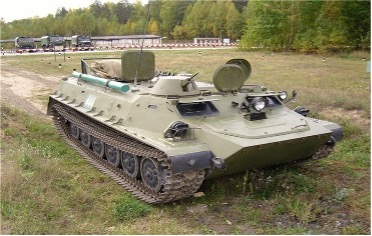
\includegraphics[width=0.95\textwidth]{src/mtlb.jpg}

\end{center}


\end{titlepage}

%====================================================
% ПУСТАЯ СТРАНИЦА 
%====================================================
\newpage
\thispagestyle{empty}
\mbox{}
\newpage

%====================================================
% ВТОРАЯ СТРАНИЦА 
%====================================================

\clearpage
% \thispagestyle{plain}

\begin{center}

\logo

\vspace{1cm}

{\Large\bfseries
Техническое обслуживание\\
легкого многоцелевого гусеничного транспортера-тягача МТЛБ
}

\vspace{1.5cm}

Учебное пособие

\vfill

\end{center}

\begin{flushright}
Рассмотрено и одобрено\\
на заседании военного учебного центра\\
Протокол №\rule{1.5cm}{0.4pt} от \rule{4cm}{0.4pt} 2026 г.\\
\end{flushright}

\vfill

\begin{center}
Санкт-Петербург
\end{center}

%====================================================
% СТРАНИЦА С АННОТАЦИЕЙ
%====================================================
\clearpage
\thispagestyle{empty}

\vspace*{\fill}
{
    % {\large\bfseries АННОТАЦИЯ} % Раскомментируйте, если нужен заголовок
    
    \noindent
    В учебном пособии рассмотрены вопросы периодичности и объема работ по техническому обслуживанию легкого многоцелевого гусеничного транспортера-тягача МТЛБ. Дано иллюстрированное сопровождение текстового материала.
    
    \medskip

    \noindent
    Учебное  пособие предназначено для студентов, проходящих военную подготовку по программам сержантов и солдат запаса, а также может быть использовано профессорско-преподавательским составом при подготовке и проведении занятий.
    
    \medskip
    
    \noindent
    Авторский коллектив: подполковник запаса Бахуревич~В.С., подполковник запаса Фирсов~О.А.
    
    \medskip
    
    \noindent
    Под общей редакцией генерал-майора запаса Глинина~В.Н.
    
    \medskip
    
    \noindent
    Авторский коллектив выражает искреннюю благодарность курсанту Гребенкину~И.А. за редакторские замечания, а также за профессиональную техническую подготовку и верстку настоящего издания.
}

\vspace*{\fill}

\clearpage
\tableofcontents

\chapter*{Введение}
\addcontentsline{toc}{chapter}{Введение}

Настоящее учебное пособие предназначено для~изучения правильной организации и~проведения технического обслуживания легких многоцелевых гусеничных транспортеров-тягачей МТЛБ. 

Техническое обслуживание транспортера-тягача (рис.~\ref{mtlb1}) включает следующие виды: 

\begin{itemize}

    \item контрольный осмотр перед выходом из~парка; 
    \item контрольный осмотр в~пути (на~привалах и~остановках); 
    \item ежедневное техническое обслуживание; 
    \item техническое обслуживание №1 (ТО-1) через \range{800}{1000}~км пробега;
    \item техническое обслуживание №2 (ТО-2) через \range{2400}{3000}~км пробега;

\end{itemize}

\begin{figure}[]
    \centering
    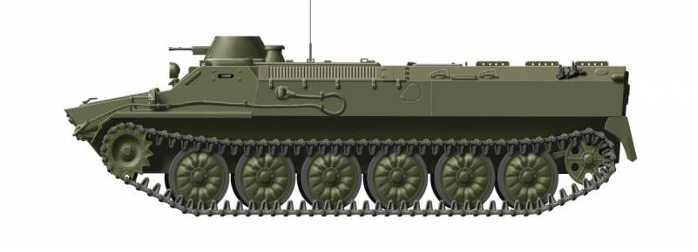
\includegraphics[width=\textwidth]{src/mtlb_1.png}
    \caption{Транспортер-тягач МТ-ЛБ}
    \label{mtlb1}
\end{figure}

Кроме контрольных осмотров и~технических обслуживании  №1 и~2 проводятся дополнительные работы по~уходу и~сбережению транспортеров-тягачей: 

\begin{itemize}
    \item один раз в~месяц в~парковые дни;
    \item при~переводе транспортеров-тягачей на~сезонную эксплуатацию;
    \item при~содержании транспортеров-тягачей в~консервации.
\end{itemize}

В~пособие предусмотрены дополнительные операции по~техническому обслуживанию при~эксплуатации транспортеров-тягачей в~районах Крайнего Севера, в~пустынно-песчаных и~горных районах, а~также в~период распутицы.


Учебное пособие содержит:
\begin{itemize}
    \item перечень операций по~каждому виду осмотра и~технического обслуживания; 
    \item указания о~составе исполнителей, объеме трудовых затрат и~времени простоя транспортеров-тягачей при~проведении осмотров и~обслуживании;
    \item перечень операций по~консервации транспортеров-тягачей и~техническому обслуживанию их в~консервации; 
    \item технологические карты на~наиболее сложные операции по~техническому обслуживанию.
\end{itemize}

В~табл.~\ref{worktime} и \ref{worktime2} даны трудовые затраты и~время простоя транспортеров-тягачей при~контрольных осмотрах и~техническом обслуживании. 

Верхние пределы трудозатрат и~времени простоя относятся к~выполнению технического обслуживания с~полным объемом регулировочных работ, в~знаменателе~--- то~же, но~при~эксплуатации транспортеров-тягачей в~тяжелых дорожных условиях (периоды весенней и~осенней распутицы, работы после форсирования водных преград). 


\begin{sidewaystable}
    \footnotesize
    {
    \newcommand{\length}{1.97cm}
    \newcommand{\longlength}{5cm}
    \centering
    \begin{tabular}{|m{\longlength}|>{\tc}m{\length}|>{\tc}m{\length}|>{\tc}m{\length}|>{\tc}m{\length}|>{\tc}m{\length}|}
        \hline
        \multirow{2}{\longlength}{\centering Вид работ} & \multicolumn{5}{c|}{\textbf{Трудозатраты, \textit{чел.-час}}} \\ 
        \cline{2-6}
        & \textbf{механика-водителя} & \textbf{механика} & \textbf{электрика} & \textbf{слесаря} & \textbf{общие} \\
        \hline
        Контрольный осмотр перед выходом из~парка & 27--40~мин &~--- &~--- &~--- & 27--40~мин  \\
        \hline
        Контрольный осмотр в~пути & 20--30~мин &~--- &~--- &~--- & 27--40~мин  \\
        \hline
        Ежедневное техническое обслуживание & 
            \begin{tabular}{c}
                 1,2--2,3 \\
                 \hline
                 1,6--2,7
            \end{tabular} &~--- &~--- &~--- & 
            \begin{tabular}{c}
                 1,2--2,3 \\
                 \hline
                 1,6--2,7
            \end{tabular}
            \\
        \hline
        Техническое обслуживание №1 &
            \begin{tabular}{c}
                 3,8--9,1 \\
                 \hline
                 4,7--9,4
            \end{tabular} &
            \begin{tabular}{c}
                 1,2--1,6 \\
                 \hline
                 2,1--2,4
            \end{tabular} &
            \begin{tabular}{c}
                 0,5--0,7 \\
                 \hline
                 1,9--2,2
            \end{tabular} &
            \begin{tabular}{c}
                 1,5--1,7 \\
                 \hline
                 1,9--1,2
            \end{tabular} &
            \begin{tabular}{c}
                 7--13,1 \\
                 \hline
                 9,6--15
            \end{tabular} \\
        \hline
        Техническое обслуживание №2 &
            \begin{tabular}{c}
                 10,2--17,1 \\
                 \hline
                 12,7--17,6
            \end{tabular} &
            \begin{tabular}{c}
                 4--5 \\
                 \hline
                 4,6--5,8
            \end{tabular} &
            \begin{tabular}{c}
                 1,2--1,7 \\
                 \hline
                 2--3
            \end{tabular} &
            \begin{tabular}{c}
                 2,9--3,9 \\
                 \hline
                 3,7--4,8
            \end{tabular} &
            \begin{tabular}{c}
                 18,3--28,3 \\
                 \hline
                 23--31,2
            \end{tabular} \\
        \hline
        Подготовка к~летнему периоду эксплуатации (дополнительно к~ТО-1 и~ТО-2) & \range{2}{2,2} &~--- & 0,5 & 1 & \range{3,5}{3,7} \\
        \hline
        Подготовка к~зимнему периоду эксплуатации (дополнительно к~ТО-1 и~ТО-2) & \range{4,6}{4,9} & 0,5 & 0,5 & 2,1 & \range{7,7}{8} \\
        \hline
    \end{tabular}
    \caption{Трудозатраты на~контрольные осмотры и~техническое обслуживание}
    \label{worktime}
    }
    \textit{Примечания:} 
    \begin{itemize}
        \item \textit{В~трудозатраты на~контрольный осмотр перед выходом из~парка не~включено время на~пуск и~прогрев двигателя при~низких температурах воздуха.} 
        \item \textit{Трудоемкость работ по~ежедневному обслуживанию приведена без~учета времени на~уборочно-моечные работы, которое для~транспортеров-тягачей различной загрязненности составляет \range{1,5}{3}~чел.-час.} 
    \end{itemize}
\end{sidewaystable}

\begin{table}
    \newcommand{\length}{1.82cm}
    \centering
    \begin{tabular}{|m{\length}|m{\length}|m{\length}|m{\length}|m{\length}|}
        \hline
        \multirow{2}{\length}{\tc ЕТО} & \multirow{2}{\length}{\tc ТО-1}  & \multirow{2}{\length}{\tc ТО-2} & \multicolumn{2}{m{\dimexpr \length * 2 + 12pt \relax}|}{\tc Подготовка к~периоду эксплуатации} \\ 
        \cline{4-5}
        &&& \tc летнему & \tc зимнему \\
        \hline
        \tc \range{1,2}{2,7} & \tc\range{3,8}{9,4} & \tc\range{10,2}{17,6} & \tc 3,7 & \tc 8 \\ 
        \hline
    \end{tabular}
    \caption{Простой транспортера-тягача при~техническом обслуживании и~при~подготовке его к~эксплуатации в~летний и~зимний периоды, \textit{ч}}
    \label{worktime2}
\end{table}

При~определении времени на~техническое обслуживание заместитель командира по~технической части (начальник автотракторной службы) должен учитывать техническое состояние и~потребность в~проведении регулировок тех или~иных агрегатов и~механизмов транспортеров-тягачей. 




\chapter{Техническое обслуживание}
%====================================================
% Техническое обслуживание
%====================================================

При техническом обслуживании отдельные исполнители выполняют следующие работы:
\begin{itemize}
    \item \textbf{механик-водитель}~--- мойку и чистку транспортера-тягача, подтяжку креплений и смазку агрегатов, узлов и механизмов, отдельные регулировки механизмов (совместно с механиком), перевод агрегатов на сезонные (зимние и летние) сорта горючего, смазки и охлаждающей жидкости, подготовку средств подогрева двигателя, обогрева, утепления и вентиляции;
    \item \textbf{механик}~--- проверку работы, регулировку и устранение неисправностей агрегатов и механизмов транспортера-тягача, промывку систем смазки и охлаждения двигателя, проверку работы на ходу после технического обслуживания и устранения замеченных недостатков; 
    \item \textbf{электрик}~--- проверку состояния электрооборудования и его крепление, устранение неисправностей в работе электрооборудования;  
    \item \textbf{слесарь}~--- подтяжку креплений агрегатов и механизмов, операции по смазке (совместно с механиком-водителем и его помощником). 
    
\end{itemize}

Для выполнения работ по ежедневному обслуживанию в помощь механику-водителю выделяются 1-2 чел. 

Операции по техническому обслуживанию транспортеров-тягачей выполняются с помощью индивидуальных (возимых) комплектов ЗИП и дополнительного инструмента и приспособлений, необходимых для работ по ТО-1 и ТО-2, входящих в комплекты Пункта технического обслуживания.

\section{Контрольный осмотр}

Контрольный осмотр~--- это совокупность операций, проводимых экипажем (механиком-водителем) в целях определения степени готовности объекта к применению по назначению. 

Цель контрольного осмотра (КО)~--- проверка технического состояния перед выполнением предстоящей задачи и устранение выявленных недостатков.

Контрольный осмотр является первичным видом контроля технического состояния.  Он проводится: 
\begin{itemize}
    \item при хранении объекта~--- ежемесячно;
    \item при использовании~--- перед выходом из парка, в пути (на привалах и длительных остановках), перед преодолением водной преграды и после ее преодоления. 
\end{itemize}

Продолжительность проведения контрольного осмотра:
\begin{itemize}
    \item перед выходом~--- \range{15}{20}~мин;
    \item на привалах~--- \range{10}{15}~мин.
\end{itemize}


\subsection{Содержание работ и технические условия перед выходом из парка}

\begin{figure}[]
    % // TODO нечитаемый текст на картинке
    \centering
    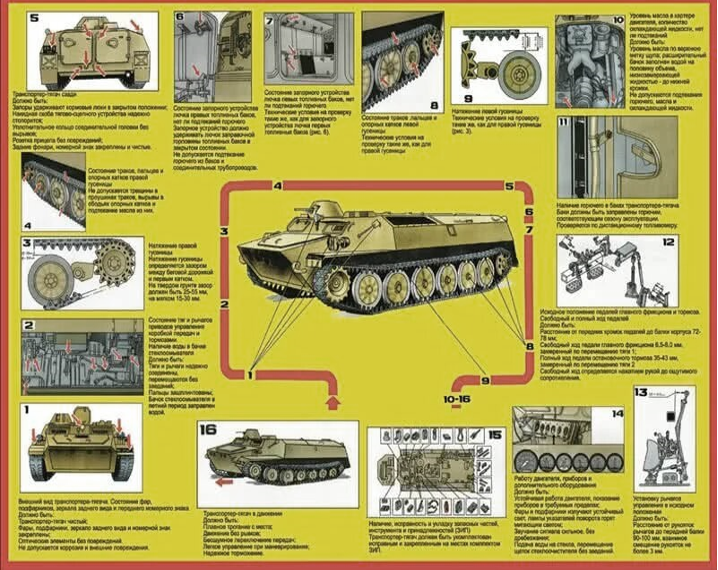
\includegraphics[width=\textwidth]{src/pic_1.png}
    \caption{Содержание работ и технические условия перед выходом из парка}
    \label{pic1}
\end{figure}


\subsubsection{По транспортеру-тягачу}

\begin{enumerate}
    \item Осмотреть транспортер-тягач, при необходимости удалить пыль, влагу, снег. 
    \item Установить аккумуляторные батареи, если они были сняты. 
    \item Проверить наличие и затяжку крышек люков в корпусе и на днище (после длительного перерыва в эксплуатации). 
\end{enumerate}

\subsubsection{По двигателю и его системам}

\begin{enumerate}
    \item Проверить: 
        \begin{itemize}
            \item уровень масла в картере двигателя (уровень масла должен быть по метке «В» на щупе); 
            \item уровень топлива в баках по топливомерной трубке, расположенной за сиденьем механика-водителя справа; 
            \item уровень охлаждающей жидкости (при заправке водой уровень должен быть до половины объема расширительного бачка, а при заправке низкозамерзающей жидкостью - по нижнюю кромку расширительного бачка); 
            \item нет ли подтекания охлаждающей жидкости, топлива или масла из радиаторов, баков, в местах соединений со шлангами, через сливные краники, в местах соединения трубопроводов и из фильтров (проверять после прогрева двигателя до температуры охлаждающей жидкости \celc{50}); обнаруженные подтекания устранить, а подтеки вытереть насухо; 
            \item уровень масла в топливном насосе и регуляторе, для чего вывернуть масляный щупг тщательно протереть его и установить во втулку до упора в резьбу. 
        \end{itemize}

    \item Пустить двигатель, на минимальных оборотах холостого хода (\range{450}{550}~об/мин) поработать \range{1}{2}~мин, увеличивая обороты, прогреть двигатель до температуры не ниже \celc{40}, прослушать его работу на разных оборотах коленчатого вала: дымления и посторонних шумов не должно быть.
    \item Проверить показания контрольно-измерительных приборов (масляных манометров системы смазки двигателя и главной передачи, манометра пневмосистемы и вольтамперметра). 
        
    \textbf{Показания должны быть:}
        \begin{itemize}
            \item давление масла в системе смазки двигателя на минимальных оборотах коленчатого вала не менее 1~кгс/см$^2$, при номинальных \range{4}{7}~кгс/см$^2$; 
            \item давление масла в главной передаче при эксплуатационных оборотах не менее 1,5~кгс/см$^2$; 
            \item давление воздуха в пневмосистеме \range{6}{7}~кгс/см$^2$; 
            \item величина зарядного тока (по амперметру) при номинальных оборотах коленчатого вала от 5 до 35~ампр. (в зависимости от заряженности аккумуляторных батарей). 
        \end{itemize}
\end{enumerate}


\subsubsection{По агрегатам, механизмам, системам}
\begin{enumerate}
    \item Проверить: 

\begin{itemize}
    \item исправность фар, приборов освещения и светосигнального устройства, звукового сигнала, сигнала «Стоп»; 
    \item исправность стеклоочистителя; 
    \item состояние и действие жалюзей радиатора; 
    \item нет ли утечки воздуха в пневмосистеме; 
    \item работу приводов управления и механизмов при переключении передач и поворотах транспортера-тягача (на ходу). 
\end{itemize}
\end{enumerate}


\subsubsection{По оборудованию и принадлежностям}
\begin{enumerate}
    \item Проверить:
    \begin{itemize}
        \item крепление шанцевого инструмента, ЗИП и огнетушителей; 
        \item состояние тягово-сцепного прибора; 
        \item плотность соединения соединительной головки со шлангом тормозной системы прицепа при полностью открытом разобщительном кране (при эксплуатации без прицепа кран должен быть закрыт). 
    \end{itemize}
\end{enumerate}

\subsubsection{Дополнительные работы, проводимые при эксплуатации зимой и в районах Крайнего Севера}

\begin{enumerate}
    \item Поставить аккумуляторные батареи. 
    \item Перед прогревом двигателя проверить, не застыла ли низкозамерзающая жидкость. Подогревать двигатель в строгом соответствии с заводской инструкцией. 
    \item При температуре воздуха ниже минус \celc{25} в главной передаче, бортовых передачах, ступицах опорных катков и направляющих колес применять масло МТ-14п. 
    \item Перед маршем по снежной целине и безлесной местности проверить исправность приспособлений для самовытаскивания и буксирных приспособлений. 
    \item Уложить бревно на транспортер-тягач. 
\end{enumerate}

\subsubsection{Дополнительные работы, проводимые при эксплуатации в горных районах:}

\begin{enumerate}
    \item Проверить наличие и исправность горных приспособлений (дополнительные грунтозацепы и др.). 
\end{enumerate}



\subsection{Содержание работ и технические условия в пути (на привалах и остановках)}
\subsubsection{По двигателю и его системам}
\begin{enumerate}
    \item Проверить: 
        \begin{itemize}
            \item уровень масла в картере двигателя, топлива в баках и охлаждающей жидкости в расширительном бачке; при необходимости дозаправить; 
            \item нет ли подтеканий охлаждающей жидкости, топлива, масла; обнаруженную течь устранить, а вытекшую смазку вытереть насухо. 
        \end{itemize}
\end{enumerate}

\subsubsection{По силовой передаче, ходовой части и механизмам управления}
\begin{enumerate}
    \item Проверить: 
    \begin{itemize}
        \item нагрев картеров бортовых передач, ступиц направляющих колес и опорных катков; нагрев считается нормальным, если не вызывает ощущения ожога ладони руки; 
        \item состояние траков и пальцев гусеничных цепей; траки, имеющие трещины, опасные для дальнейшей работы, и поломанные пальцы должны быть заменены; 
        \item натяжение гусеничных цепей; при необходимости отрегулировать, их натяжение (см. технологическую карту №\ref{techcard25}). 
    \end{itemize}
\end{enumerate}


\subsubsection{По оборудованию и принадлежностям}
\begin{enumerate}
    \item Проверить: 
    \begin{itemize}
        \item надежность сцепки с прицепом, исправность тягово-сцепного прибора и плотность соединения соединительной головки со шлангом тормозной системы; 
        \item состояние и крепление груза в кузове и на прицепе; 
        \item крепление ЗИП, шанцевого инструмента и огнетушителей; 
        \item состояние ходовой части прицепа. 
    \end{itemize}
\end{enumerate}

\subsubsection{Дополнительные работы, проводимые при эксплуатации зимой и в районах Крайнего Севера}
\begin{enumerate}
    \item Во время стоянки транспортера-тягача и особенно при сильном морозе периодически пускать и прогревать двигатель. 
    \item Сбить снег или лед, намерзший на беговых дорожках гусениц. 

\end{enumerate}



\section{Ежедневное техническое обслуживание}
Ежедневное техническое обслуживание (ЕТО) проводится с целью контроля исправного состояния машины, обеспечивающего безопасность движения, а также заправки топливом, маслом и охлаждающей жидкостью и поддержания внешнего вида, а также обеспечении последующей надежной работы при пробеге не менее \range{250}{300}~км. Ежедневное техническое обслуживание проводится экипажами (механиками-водителями) с участием специалистов подразделений технического обеспечения в конце дня после каждого выхода из парка независимо от пробега (в конце суток боевых действий).

Ежедневное техническое обслуживание включает:
\begin{itemize}
    \item общий контроль технического состояния машины; 
    \item дозаправку ГСМ, боеприпасами (во время боевых действий);
    \item мойку (чистку);
    \item проверку комплектности.
\end{itemize}

Последовательность выполнения работ ежедневного технического обслуживания определяется командиром в соответствии с условиями проведения работ, наличием экипажа и имеющимся временем. 

В первую очередь выполняются работы, которые влияют на боеготовность образцов ВВТ (пополнение боеприпасов, дозаправка ГСМ и т.д.). 

В парке работы ежедневного технического обслуживания производятся в технологической последовательности прохождения машины по элементам линии технического обслуживания.

Продолжительность проведения ежедневного технического обслуживание определяется приказом МО 1998~г. и действующими инструкциями по техническому обслуживанию и составляет: \range{1,5}{2} часов.


\subsection{Содержание работ и технические условия}
\subsubsection{По транспортеру-тягачу}
\begin{enumerate}
    \item Сразу после пробега (при наличии в раме топлива, масла и воды) поставить транспортер-тягач на уклон с креном на корму или нос, открыть кингстоны для слива скопившегося топлива, масла, воды. 
    \item Осмотреть нет ли подтекания масла из агрегатов силовой передачи и ходовой части и проверить степень их нагрева. 
    \item Заправить транспортер-тягач топливом. 
    \item Проверить уровень масла и охлаждающей жидкости и при необходимости дозаправить. 
    \item Очистить и вымыть транспортер-тягач снаружи, убрать в кабине и кузове, вытереть насухо все узлы, стекла кабины, фар, прожектора, задних фонарей и мастику аккумуляторных батарей; протереть днище рамы и закрыть кингстоны.
    \item Проверить состояние днища (нет ли деформаций и пробоин), наличие и затяжку крышек люков. 
    \item Устранить неисправности, обнаруженные в пути и при обслуживании. 
\end{enumerate}

\subsubsection{По двигателю и его системам}
\begin{enumerate}
\item Проверить не подтекает ли охлаждающая жидкость из радиатора в местах соединений со шлангами и из сливных краников; не подтекает ли топливо и масло в местах соединений трубопроводов, из фильтров. Обнаруженные подтекания устранить, а подтеки вытереть насухо. 
\item Спустить 0,1~л топлива из фильтров грубой очистки и тонкой очистки. После этого дать двигателю поработать \range{3}{4}~мин для удаления воздушных пробок.
\item Проверить состояние и натяжение ремней приводов генератора, водяного насоса, компрессора и вентилятора. При необходимости отрегулировать (см. технологические карты №\ref{techcard8}, \ref{techcard9}, \ref{techcard10} и \ref{techcard11}). 

\textbf{При нажатии большим пальцем руки с усилием \range{3}{4}~кгс прогиб должен быть, \textit{мм}:}
\begin{itemize}
    \item на короткой ветви ремней привода генератора \range{10}{12}; 
    \item на середине ветви ремня привода водяного насоса \range{10}{15}; 
    \item на середине ветви ремня привода компрессора \range{5}{8};
    \item на верхней ветви ремней привода вентилятора \range{8}{14}. 
\end{itemize}

\item Проверить уровень масла в регуляторе числа оборотов и в топливном насосе. Уровень масла должен быть по верхнюю метку на щупе. При необходимости дозаправить. 
\end{enumerate}


\subsubsection{По электрооборудованию}
\begin{enumerate}
    \item Проверить крепление и, работу фар, поворотной фары-искателя, задних фонарей и звукового сигнала, включив выключатель массы. Ослабление крепежных деталей не допускается. 
    \item Через каждые 15 дней, а в жаркое время через \range{5}{6} дней, проверить уровень и плотность электролита в батареях, крепление аккумуляторных батарей и прочистить вентиляционные отверстия в них. Через каждые \range{30}{35} дней независимо от степени заряженности аккумуляторные, батареи заряжать на зарядной станции. Уровень электролита должен быть выше предохранительного щитка на \range{8}{10}~мм. 
\end{enumerate}



\begin{sidewaystable}
    \center
    \begin{tabular}{|m{5cm}|m{1.5cm}|>{\tc}m{4.5cm}|>{\tc}m{4.5cm}|}
        \hline
        \multicolumn{2}{|m{6.5cm}|}{\tc Районы эксплуатации} & Минимальная окружающая температура, \celc{} & Плотность электролита заряженных батарей при~его температуре $+$\celc{15} \\
        \hline
        \multicolumn{2}{|m{6.5cm}|}{\tc Южные} & до $-$20 & 1,25 \\
        \hline
        \multicolumn{2}{|m{6.5cm}|}{\tc Центральные} & до $-$30 & 1,27 \\
        \hline
        \multicolumn{2}{|m{6.5cm}|}{\tc Северные} & до $-$40 & 1,29 \\
        \hline
        \multirow{2}{5cm}{\tc С резко континентальным климатом} & \tc зимой && 1,31 \\
        \cline{2-4}
        & \tc летом & & 1,27 \\
        \hline
    \end{tabular}

    \caption{Плотность электролита полностью заряженных батарей для различных климатических условий эксплуатации}
    \label{electrolyte_density}

    \flushleft
    \textit{Примечания:}
    \begin{itemize}
        \itshape
        \item Степень разряженности батарей при эксплуатации зимой допускается не более 25~\%, а~летом~--- не более 50~\%.
        \item Понижение плотности электролита на 0,01 соответствует разрядке батареи примерно на \range{5}{6,25}~\%.
    \end{itemize}
\end{sidewaystable}

\newpage

\subsubsection{По силовой передаче, ходовой части и механизмам управления}
\begin{enumerate}
    \item Провернуть на \range{два}{три} оборота рукоятку оси масляного фильтра главной передачи. 
    \item Проверить: 
    \begin{itemize}
        \item состояние торсионов, траков и пальцев гусениц; 
        \item натяжение гусениц; правильность натяжения определяется по положению верхней ветви. Она должна лежать на четырех опорных катках, не касаясь первого и шестого катков. При необходимости отрегулировать (см. технологическую карту №\ref{techcard25}); 
        \item состояние резиновых бандажей опорных катков;
        \item крепление гидравлических амортизаторов; 
        \item нет ли утечки воздуха из пневмосистемы. 
    \end{itemize}
\end{enumerate}


\subsubsection{По оборудованию и принадлежностям}
\begin{enumerate}
    \item После возвращения из рейса, открыть кран отбора воздуха и слить конденсат из баллонов пневмосистемы. 
    \item Проверить: 
    \begin{itemize}
        \item состояние и крепление тягово-сцепного прибора; 
        \item состояние вооружения (в соответствии с наставлением по вооружению) и укладку боеприпасов (МТЛБ); 
        \item состояние смотровых приборов (МТЛБ) и при необходимости очистить их; 
        \item укладку и крепление ЗИП; 
        \item крепление огнетушителей. 
    \end{itemize}
\end{enumerate}


\subsubsection{По смазке}
\begin{enumerate}
    \item Смазать агрегаты и механизмы транспортера-тягача согласно таблице смазки.
\end{enumerate}

\begin{figure}[h]
    \centering
    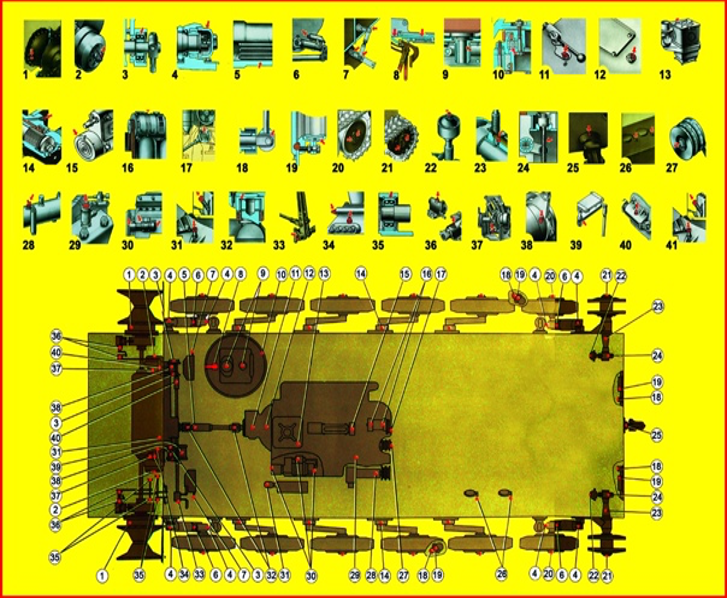
\includegraphics[width=\textwidth]{src/lubricant.png}
    \caption{Схема смазки}
    \label{lubricant}
\end{figure}


\subsubsection{Дополнительные работы, проводимые при эксплуатации зимой и в районах Крайнего Севера}
\begin{enumerate}
    \item Если предвидится длительный перерыв в эксплуатации транспортера-тягача при хранении его на открытом воздухе или в неотапливаемом помещении при температуре наружного воздуха ниже минус \celc{15}, снять аккумуляторные батареи и поставить их в отапливаемое помещение. 
    \item Проверить исправность средств подогрева. 
    \item Открыть нижнюю пробку камеры горения отопительно-вентиляционной установкой. ОВ-65 и слить конденсат. 
    \item Проверить, нет ли воды во впускных и выпускных патрубках. 
\end{enumerate}

\subsubsection{Дополнительные работы, проводимые при эксплуатации в районах песчано-пустынной и на сильно запыленной местности}
\begin{enumerate}
    \item Очистить поверхность радиатора от песка и пыли. 
    \item Через \range{4}{5} дней проверить работу паровоздушного клапана пробки расширительного бачка. 
    \item Через \range{25}{30}~ч работы двигателя очистить и промыть фильтрующий элемент, бункер и циклоны воздухоочистителя (см. технологическую карту №\ref{techcard7}).
    \item Очистить и промыть атмосферные фильтры в пробках заливных 
горловин. 
\end{enumerate}

\subsubsection{Дополнительные работы, проводимые при эксплуатации в горных районах}
\begin{enumerate}
    \item Если ожидается понижение температуры воздуха ниже нуля, слить воду из системы охлаждения (чтобы меньше было накипи эту же воду целесообразно вновь использовать для заправки системы охлаждения). 
    \item Один раз в три дня проверять уровень электролита в батареях.
\end{enumerate}

\subsubsection{Дополнительные работы, проводимые после преодоления бродов (водных преград)}
\begin{enumerate}
    \item Смазать подшипники механизма выключения фрикционов механизмов поворота. 
    \item Проверить наличие воды, в масле бортовых передач, главной передаче, опорных катков и направляющих колес. При обнаружении следов воды (масло имеет серый цвет, повышенный уровень масла, наличие воздушных пузырьков) масло заменить. 
    \item При необходимости промыть систему водооткачивания заливкой воды через водовыбрасывающий патрубок, слив воды -  через кингстоны, не включая водооткачивающий насос. 
\end{enumerate}

\subsubsection{Дополнительные работы, проводимые при эксплуатации в условиях грязных дорог и распутицы}
\begin{enumerate}
    \item По окончании периода интенсивной ежедневной эксплуатации, но не более чем через 500 км пробега, проверить уровень масла в картерах бортовых передач и при обнаружении воды или грязи в масле, сменить его. 
    \item В случае повышенного нагрева охлаждающей жидкости системы охлаждения двигателя - снять жалюзи, очистить и промыть водой поверхность радиатора от грязи.

\end{enumerate}


\section{Техническое обслуживание №1}
Техническое обслуживание №1 (ТО-1) предназначено для детальной проверки технического состояния машины, выявления и устранения неисправностей, обеспечения безотказной работы машины до очередного номерного обслуживания.

Техническое обслуживание №1 выполняется в пункте технического обслуживания и ремонта (ПТОР) для гусеничных тягачей и транспортеров~--- через \range{800}{1000}~км. 

Техническое обслуживание №1 включает объем ЕТО и ряд дополнительных операций по контрольной диагностике, смазке, проверке крепления, исправности и укомплектованности механизмов и агрегатов, выполнения необходимых регулировок и устранению обнаруженных неисправностей. Они в основном выполняются без разборки агрегатов.

Техническое обслуживание №1 проводится личным составом, закрепленным за вооружением и техникой, с привлечением сил и средств технического обеспечения соединения (части, подразделения). Организует командир подразделения.

Средняя трудоемкость технического обслуживания №1 (без учета уборочно-моечных работ) для гусеничных машин составляет 10 чел./час. Простой машин на техническом обслуживании №1 для гусеничных машин~--- 6 часов. 

\subsection{Содержание работ и технические условия}
Выполнить все операции, указанные для ежедневного технического обслуживания. Дополнительно провести следующие работы: 


\subsubsection{По двигателю и его системам}
\begin{enumerate}
    \item Проверить крепление: 
    \begin{itemize}
        \item опор двигателя
        \item топливных баков
        \item натяжного ролиБрезент должен быть закреплен так, чтобы он не соприкасался с землей, не раздувался ветром; на поверхности брезента нежка 
        \item масляного и водяного насосов
        \item топливного насоса высокого давления
        \item радиатора
        \item других приборов систем питания, смазки, охлаждения.
    \end{itemize}
    Ослабление креплений не допускается. При необходимости подтянуть.
    
    \item Проверить:
        \begin{itemize}
            \item состояние и герметичность трубопроводов, агрегатов и приборов систем смазки, питания и охлаждения; при необходимости неисправности устранить: 
            \item регулировку привода управления топливным насосом; 
            \item работу механизма останова двигателя; 
            \item состояние паровоздушного клапана расширительного бачка (загрязнение и легкость хода штока клапана); в случае заедания промыть клапан горячей водой; 
            \item плотность низкозамерзающей жидкости (в зимнее время). 
            
            \textbf{Плотность жидкости «40» должна быть \range{1,068}{1,073}, а жидкости «65»~--- \range{1,085}{1,090}.}
        \end{itemize} 
    \item Промыть фильтр центробежной очистки масла (см. технологическую карту №\ref{techcard5}). 
    \item Промыть фильтр грубой очистки масла (через одно ТО-1), (см.  технологическую карту №\ref{techcard4}), очистить и промыть через 50 ч работы двигателя фильтрующий элемент, бункер и циклоны воздухоочистителя (см. технологическую карту №\ref{techcard7}). 
    \item При работе в пыльных условиях очистить сердцевину радиатора системы охлаждения от пыли и грязи. Промыть и продуть сжатым воздухом сапун топливного насоса высокого давления. 
\end{enumerate}

\subsubsection{По электрооборудованию}
\begin{enumerate}
    \item Проверить и при необходимости очистить зажимы аккумуляторных батарей от окиси, затянуть и слегка смазать, 
    \item Проверить: 
    \begin{itemize}
        \item крепление генератора, стартера, реле-регулятора и при необходимости подтянуть; 
        \item состояние всех контактов электроприборов, при необходимости зачистить и затянуть крепления. 
    \end{itemize}
\end{enumerate}

\subsubsection{По силовой передаче и ходовой части}
\begin{enumerate}
    \item Проверить: 
        \begin{itemize}
            \item крепление венцов ведущих колес, карданного вала промежуточного редуктора, гаек балансиров, колпаков опорных катков, направляющих и ведущих колес, корончатых гаек коленчатых осей и ободьев направляющих колес, конических пружин упоров, приспособлений для снегоочистителя, механизмов и приводов управления транспортера-тягача, при необходимости подтянуть крепления и зашплинтовать; 
            \item крепление тормозного крана и пневмокамер тормозов, открыв люк главной передачи. 
            \item регулировку механизмов поворота и остановочных тормозов, при необходимости отрегулировать (см. технологические карты №\ref{techcard23} и \ref{techcard19}); 
            \item исправность предохранительного клапана пневмосистемы; при повышении давления больше 7,5 кгс/см$^2$ клапан снять, промыть и отрегулировать; 
            \item шплинтовку шарнирных соединений приводов управления транспортера-тягача. 
        \end{itemize}
    \item Слить отстой из масляного фильтра главной передачи (сразу после возвращения из рейса в парк). 
    \item Проверить и при необходимости отрегулировать полный и свободный ход педали главного фрикциона (см. технологическую карту №\ref{techcard18}).
\end{enumerate}

\subsubsection{По оборудованию и принадлежностям}
\begin{enumerate}
    \item Проверить состояние огнетушителей путем взвешивания, при необходимости подзарядить (минимально допустимый вес заряда огнетушителей ОУ-2 1,25 кг). 
    \item Проверить герметичность корпуса.
\end{enumerate}

\subsubsection{По агрегатам и механизмам}
\begin{enumerate}
    \item Проверить работу механизмов управления при переключении передач и на поворотах (на ходу транспортера-тягача); при необходимости отрегулировать их (см. технологические карты №\ref{techcard19}, \ref{techcard20}, \ref{techcard21}, \ref{techcard22}, \ref{techcard23} и \ref{techcard24}). 
\end{enumerate}

\subsubsection{По смазке}
\begin{enumerate}
    \item Смазать агрегаты и механизмы транспортера-тягача согласно таблице смазки.
\end{enumerate}

\subsubsection{Дополнительные работы, проводимые при эксплуатации в песчано-пустынных районах и на сильно запыленной местности}
\begin{enumerate}
    \item Очистить и смазать посадочные места коленчатых осей направляющих колес и гнезда кронштейнов (при затрудненном проворачивании коленчатых осей). 
    \item После 25-30 ч работы двигателя очистить фильтрующие элементы воздухоочистителя (промыть в дизельном топливе) от пыли, грязи и промаслить фильтрующие элементы в масле МТ-16п, смазать войлочные уплотнители и прокладки.
\end{enumerate}


\section{Техническое обслуживание №2}
Техническое обслуживание №2 (ТО-2) предназначено для обеспечения безотказной работы агрегатов, узлов и систем машины в пределах установленных норм, снижения интенсивности износа деталей, выявления и предупреждения отказов и неисправностей путем своевременного проведения контрольно-диагностических, смазочных, крепежных, регулировочных и других работ.

Техническое обслуживание №2  выполняется также в ПТОР для гусеничных тягачей и транспортеров через \range{2400}{3000}~км,

Техническое обслуживание №2  включает объем работ, технического обслуживания №1 и, кроме того, установленные нормативно-технической (эксплуатационной) документацией дополнительные операции, для выполнения которых требуется частичная или полная разборка отдельных агрегатов, узлов и аппаратуры с заменой сборочных единиц, отработавших или отслуживших установленный ресурс и не соответствующих требуемым пара¬метрам.

Этим обслуживанием завершается цикл технического обслуживания машины.

Техническое обслуживание №2  выполняется специалистами ПТОР при участии механика-водителя обслуживаемой машины.

Средняя трудоемкость технического обслуживания №2  составляет: для гусеничных машин соответственно 13 и 25 чел./час. Простой машин при техническом обслуживании №2  планируется из расчета-гусеничных машин~--- 12 ч.

Исполнители~--- механик, механик-водитель, электрик и слесарь. 

\subsection{Содержание работ и технические условия}
Выполнить все операции, указанные для технического обслуживания №1. Дополнительно провести следующие работы:

\subsubsection{По двигателю и его системам}
\begin{enumerate}
    \item Проверить: 
        \begin{itemize}
            \item угол опережения впрыска топлива, при необходимости (через одно ТО-2) отрегулировать (см. технологическую карту №\ref{techcard13}); 
            \item зазоры клапанного механизма, при необходимости отрегулировать; (зазоры у впускного и выпускного клапанов должны быть \range{0,25}{0,30}~мм, см.~технологическую карту №12); 
            \item положение педали подачи топлива, при необходимости отрегулировать; при минимальной подаче топлива педаль должна находиться в верхнем крайнем положении (рычажок регулятора двигателя должен касаться переднего регулировочного болта), а при максимальной подаче~--- в нижнем крайнем положении при упоре в регулировочный болт (рычажок регулятора устанавливается в крайнее заднее положение, зазор до упора должен быть от 0 до 1,2~мм~--- он регулируется тягой регулятора или упорным болтом, см. технологическую карту №\ref{techcard16}). 
        \end{itemize}
    \item Заменить элементы фильтров грубой и тонкой очистки топлива и промыть корпусы фильтров (см. технологические карты №\ref{techcard1} и \ref{techcard2}). 
    \item Подтянуть гайки крепления головок цилиндров, момент затяжки должен быть 22-24 кГм. 
    \item Снять форсунки с двигателя и проверить их работу на стенде (см. технологическую карту №\ref{techcard15}). 
    \item Снять и проверить топливный насос высокого давления, при необходимости (через 2000 ч работы двигателя, а на новом двигателе первый раз через 1200 ч) отрегулировать (см. технологическую карту №\ref{techcard14}). 
    \item Снять и промыть (через одно ТО-2) топливные баки (см. технологическую карту №\ref{techcard3}). 
    \item Снять и промыть (через одно ТО-2) в профильтрованном дизельном топливе сапун двигателя путем многократного погружения его в топливо, после чего продуть сжатым воздухом. 
\end{enumerate}


\subsubsection{По электрооборудованию}
\begin{enumerate}
    \item Проверить: 
        \begin{itemize}
            \item состояние (после истечения гарантийного срока) коллектора, щеток, щеткодержателей генератора и стартера, продуть генератор и стартер сжатым воздухом, при необходимости зачистить поверхность коллекторов от нагара; 
            \item крепление выключателя массы, блока предохранителей, контрольных приборов; 
            \item установку фар и при необходимости отрегулировать; 
            \item контакты пускового реле стартера и в случае подгорания зачистить; 
            \item изоляцию проводов. 
        \end{itemize}
    \item Снять аккумуляторные батареи, проверить и при необходимости зарядить
\end{enumerate}

\subsubsection{По силовой передаче и ходовой части}
\begin{enumerate}
    \item Проверить: 
        \begin{itemize}
            \item крепление главной передачи 
            \item бортовых передач 
            \item ведущих колес 
            \item зубчатых муфт и тормозных барабанов. 
        \end{itemize}
        Гайки и болты должны быть затянуты до отказа. 
        
    \item Проверить и при необходимости отрегулировать: 
        \begin{itemize}
            \item величину полного хода педали остановочного тормоза - определяется перемещением тяги тормозного крана (см. технологическую карту №\ref{techcard18}); 
            \item регулировку привода коробки передач (см. технологическую карту №\ref{techcard17}); 
            \item выставку рычагов управления (см. технологическую карту №\ref{techcard20}); 
            \item свободный ход хвостовиков поводковых коробок механизмовповорота (см. технологическую карту №\ref{techcard21}). 
        \end{itemize}
\end{enumerate}

\subsubsection{По оборудованию и принадлежностям}
\begin{enumerate}
    \item Проверить крепление:  
    \begin{itemize}
        \item контрольных приборов и проводов на щитке водителя; 
        \item лебедки, реверса редуктора, карданных шарниров и датчика предохранительного устройства отключения привода лебедки; гайки и болты должны быть затянуты до упора; 
        \item котла подогревателя, а в зимний период и его работу. 
    \end{itemize}
    \item Снять и промыть (через одно ТО-2) заборники водооткачивающей системы. 
    \item Проверить работу установки ТКБ-01 и переговорного устройства в соответствии с действующими инструкциями.  
    \item Проверить наличие, состояние и крепление ЗИП. 
\end{enumerate}

\subsubsection{По смазке}
\begin{enumerate}
    \item Смазать агрегаты и механизмы транспортера-тягача согласно таблице смазки. 
\end{enumerate}


\subsubsection{Проверка контрольным пробегом}
\begin{enumerate}
    \item Контрольным пробегом на расстояние \range{1}{1,5}~км проверить работу агрегатов и механизмов транспортера-тягача после технического обслуживания №2. При этом транспортер-тягач должен удовлетворять следующим требованиям: 
    \begin{itemize}
        \item двигатель должен развивать достаточную мощность. Путь разгона на IV-й передаче в коробке передач на ровном твердом грунте со скорости 12 км/ч до скорости 25 км/ч не должен превышать 50 м; 
        \item при изменении положения педали или ручного привода подачи топлива двигатель должен соответственно увеличивать или уменьшать обороты коленчатого вала, но не останавливаться; 
        \item при перемещении любого рычага управления в среднее положение транспортер-тягач должен плавно поворачиваться в соответствующую сторону. При перемещении рычага в крайнее зад нее положение на 1-й передаче в коробке передач транспортер-тягач должен разворачиваться с минимальным радиусом поворота, при возвращении рычагов в исходное положение~--- должен двигаться в прямом направлении; 
        \item при включении главного фрикциона не должны прослушиваться стуки и шумы, свидетельствующие о неисправности подшипника выключения фрикциона; 
        \item переключение передач должно быть бесшумным и не должно требовать применения больших усилий; 
        \item при нажатии на тормозную педаль или при оттягивании рычагов управления в заднее крайнее положение должно происходить надежное торможение; 
        \item показания контрольных приборов должны соответствовать требованиям заводской инструкции; 
        \item сразу после остановки температура ступиц направляющих колес и опорных катков не должна превышать \range{60}{70}\celc{} (ладонь руки, приложенная к ступице, не должна испытывать ощущения ожога). 
    \end{itemize}
\end{enumerate}

\section{Дополнительные работы, проводимые один раз в месяц (в парковые дни)}
\begin{enumerate}
    \item Очистить транспортер-тягач снаружи от пыли и грязи. 
    \item Проверить: 
        \begin{itemize}
            \item нет ли подтекания топлива, масла и охлаждающей жидкости;
            \item уровень и плотность электролита в аккумуляторных батареях, протереть их поверхность, прочистить вентиляционные отверстия, а также крепление батарей; 
            \item состояние и работу приборов освещения, светомаскировочных устройств, светосигнального устройства и сигнала «Стоп». 
        \end{itemize}
    \item Устранить обнаруженные при обслуживании неисправности. 
    \item Проверить: 
    \begin{itemize}
        \item наличие, исправность и укладку ЗИП;
        \item состояние лакокрасочных покрытий и при необходимости подкрасить транспортер-тягач; 
        \item состояние и надежность крепления брезентов и тентов, при необходимости отремонтировать. 
    \end{itemize} 

\end{enumerate}
Исполнитель~--- механик-водитель.

\section{Работы, проводимые при переводе на летнюю эксплуатацию}
Характеристикой условий летнего периода эксплуатации является устойчивая температура окружающего воздуха +\celc{5} и выше. Летний период эксплуатации определяется установившейся температурой окружающего воздуха, который будет от +\celc{5} и выше.

Следовательно, этот период будет характеризоваться следующими условиями: - устойчивой температурой окружающего воздуха от +\celc{5} и выше; высокой запыленностью местности; постоянным присутствием взвешенных частиц пыли в атмосфере в сухую погоду; чрезмерной загрязненностью (заболоченностью) проезжей части грунтовых дорог после выпадения осадков.

Высокая температура окружающего воздуха вызывает повышенный нагрев агрегатов машины, испарение воды из электролита АБ, а также ухудшает условия работы экипажа.  При высокой температуре окружающего воздуха и больших нагрузках может перегреваться двигатель.

Во время летней эксплуатации машины в основном работают в условиях большой запыленности воздуха. Воздух с повышенным пылесодержанием, проникающий в узлы и агрегаты машины, повышает износы деталей, увеличивает усилия на педалях, рычагах, ухудшает условия их работы.

Большая запыленность воздуха резко снижает видимость через приборы прицеливания и наблюдения, особенно при движении в колонне.


\subsection{Содержание работ и технические условия}
Выполнить в зависимости от пробега все операции по техническому обслуживанию №1 или №2 и дополнительно провести следующие операции: 

\subsubsection{По двигателю и его системам}
\begin{enumerate}
    \item Слить низкозамерзающую жидкость из системы охлаждения в чистую посуду и сдать на склад. Промыть систему охлаждения, удалить накипь из водяной рубашки двигателя и заправить ее водой. 
    \item Промыть топливные баки и заполнить их летним сортом топлива.   Промывать без снятия баков, путем заливки и слива \range{15}{20}~л топлива.
\end{enumerate}

\subsubsection{По электрооборудованию}
\begin{enumerate}
    \item Проверить степень заряженности аккумуляторных батарей и довести плотность электролита до нормы (см. таблицу ~\ref{electrolyte_density}).
\end{enumerate}

\subsubsection{По оборудованию и принадлежностям}
\begin{enumerate}
    \item После 	длительной 	работы 	разобрать отопительно-вентиляционную установку ОВ-65, проверить состояние щеток коллектора электродвигателя, состояние датчиков и очистить, камеры сгорания и трубопроводы от нагара.
\end{enumerate}

\subsubsection{По смазке}
\begin{enumerate}
    \item Перевести все агрегаты и механизмы на летние сорта смазки, с предварительной промывкой картеров. 
\end{enumerate}

\subsubsection{По транспортеру-тягачу}
\begin{enumerate}
    \item При необходимости подкрасить или полностью окрасить транспортер-тягач. 
\end{enumerate}

Исполнители~--- механик-водитель, механик, электрик и слесарь.



\section{Работы, проводимые при переводе на зимнюю эксплуатацию} 
Эксплуатация машины в зимних условиях существенно отличается от эксплуатации в летних условиях и характеризуется в основном низкими температурами окружающего воздуха и наличием снежного покрова.

Зимние условия эксплуатации машины определяются температурой окружающего воздуха от +\celc{5} и ниже.

Из всех агрегатов влиянию низких температур наиболее подвержены двигатель, коробка передач и их системы, а также аккумуляторные батареи.

Основные трудности возникают при пуске двигателя. Его надежный пуск возможен только при определенном тепловом состоянии, которое обеспечивается разогревом остывшего двигателя и поддержанием его в разогретом состоянии в течение всего времени стоянки машины, если этого требует обстановка.

Для прогрева системы управления машиной необходимо во время прогрева двигателя несколько раз с выдержкой \range{20}{30}~с выжать и отпустить педали сцепления и остановочных тормозов.

Признаком, свидетельствующим о готовности системы управления машиной к работе, является отсутствие падения давления масла (по манометру) в системе смазки при выжиме педали главного фрикциона или педали остановочных тормозов.

\subsection{Содержание работ и технические условия}
\subsubsection{По двигателю и его системам}
\begin{enumerate}
    \item Заполнить систему охлаждения низкозамерзающей жидкостью. 
    \item Снять и проверить исправность термостатов. Для этого термостат очистить от накипи и опустить в сосуд с водой, нагретой до \range{90}{100}\celc{}. По мере остывания воды следить за температурой начала и полного закрытия клапана термостата. Начало закрытия должно быть при \range{80}{83}, полное закрытие~--- при \celc{70}. Неисправный термостат заменить новым. 
    \item Слить воду из бачка устройства для обмыва стекол кабины. 
    \item Промыть систему смазки двигателя и заправить зимним сор том дизельного масла (см. технологическую карту №\ref{techcard6}). 
    \item Промыть топливные баки и топливные фильтры, заправить их зимним сортом топлива. Не допускать разбавления дизельного топлива бензином, так как это может вызвать перебои в работе топливной аппаратуры из-за образования газовых пробок (см. технологические карты №\ref{techcard1}, \ref{techcard2} и \ref{techcard3}). 
\end{enumerate}

\subsubsection{По электрооборудованию}
\begin{enumerate}
    \item Проверить степень заряженности аккумуляторных батарей и довести плотность электролита до нормы.
\end{enumerate}

\subsubsection{По оборудованию и принадлежностям}
\begin{enumerate}
    \item Проверить исправность системы подогрева, для чего:
        \begin{itemize}
            \item проверить и при необходимости очистить от нагара внутренние поверхности котла, кожуха поддона двигателя и газоотводящих труб; 
            \item проверить состояние уплотнений газоотводящих труб; 
            \item проверить подтяжку соединительных гаек, состояние топливных трубок и исправность форсунки; 
            \item если сорвана пломба, проверить поступление топлива к топливному насосу редуктора и производительность насоса при полной подаче (за 65 оборотов рукоятки ручного привода стенда количество подаваемого топлива должно быть \range{70}{80}~см$^3$). 
        \end{itemize}
    \item Проверить работу системы обогрева транспортера-тягача (отопительно-вентиляционной установки ОВ-65) и произвести обслуживание:
        \begin{itemize}
            \item продуть сжатым воздухом установку через штуцер, сняв пробку, которая устанавливается в верхней части кожуха; 
            \item проверить и при необходимости очистить свечу накаливания фильтр-отстойник, топливные и дренажные трубки; 
            \item после длительной работы (\range{50}{60}~ч) при заметном снижении качества работы установку разобрать и очистить от нагара и грязи.
        \end{itemize}
\end{enumerate}

\subsubsection{По смазке}
\begin{enumerate}
    \item Перевести все агрегаты и механизмы на зимние сорта смазки согласно таблице смазки. В агрегатах, смазываемых маслом МТ-16п, масло не заменять. 
\end{enumerate}

\subsubsection{По транспортеру-тягачу}
\begin{enumerate}
    \item При необходимости подкрасить или полностью окрасить транспортер-тягач. 
\end{enumerate}



\chapter{Хранение транспортера-тягача}
\section{Общие положения}

Порядок постановки транспортера-тягача на~хранение, последовательность и~организация работ, выполняемых при~подготовке и~содержании транспортера-тягача на~хранение, а~также порядок снятия его с~хранения определяется Наставлением по~автотракторной службе Вооруженных Сил РФ и~Инструкцией по~хранению автотракторной техники и~имущества в~воинских частях, на~базах и~складах. 

Постановке на~хранение подлежат все транспортеры-тягачи, эксплуатация которых не~планируется на~срок более трех месяцев, а~в~особых климатических условиях~--- более одного месяца. 

В~зависимости от~срока хранения транспортера-тягача она может быть кратковременной (на~срок до~одного года) и~длительный (на~срок более одного года). 

Транспортер-тягач, подлежащий кратковременному хранению, подвергается очередному номерному техническому обслуживанию (ТО-1 или~ТО-2), при~проведении которого выполняется ряд специальных дополнительных операций по~подготовке его деталей, механизмов и~агрегатов к~консервации. 
\looseness=-1

Транспортер-тягач, подлежащий длительной хранению, подвергается техническому обслуживанию №2, при~проведении которого необходимо выполнить все работы, предусмотренные через одно ТО-2 и~при~сезонном обслуживании. Одновременно с~техническим обслуживанием выполняются дополнительные работы по~подготовке транспортера-тягача к~хранению. 
\looseness=-1

Контроль за~состоянием транспортеров-тягачей, находящихся на~хранении, и~их техническое обслуживание проводятся в~следующие сроки: 
\begin{itemize}
    \item один раз в~месяц (в~парковые дни);
    \item один раз в~шесть месяцев (при~подготовке транспортеров-тягачей к~летнему и~зимнему периодам эксплуатации); 
    \item один раз в~год (в~сухую, без~осадков, погоду).
\end{itemize}

\begin{table}[h]
    \center
    \begin{tabular}{|m{2cm}|>{\tc}m{2.5cm}|>{\tc}m{2.5cm}|>{\tc}m{2.5cm}|}
        \hline
        \multicolumn{2}{|m{4.5cm}|}{\multirow{2}{4.5cm}{\tc Вид трудозатрат}} & \multicolumn{2}{m{5cm}|}{\tc Трудозатраты на~подготовку к~консервации, \textit{чел.-час} } \\
        \cline{3-4}
        \multicolumn{2}{|c|}{} & кратко\-временную  & длительную \\
        \hline
        \multicolumn{2}{|m{4.5cm}|}{Без~учета ТО-1 и~ТО-2}  & 13,5 & 18,2 \\
        \hline
        \multirow{2}{2cm}{\centering С учетом ТО-1 и~ТО-2} & без~регулировочных работ & \range{20,5}{26,5} & \range{40,2}{54,5} \\
        \cline{2-4}
        & с~регулировочными работами & \range{23,1}{28,5} & \range{44,9}{57,2} \\
        \hline

    \end{tabular}
    \caption{Трудозатраты на~подготовку к~консервации}
    \label{worktime_conserv}
\end{table}

Кроме этого, ежегодно опробуется 50\% транспортеров-тягачей, находящихся на~длительном хранении, из~них: 30\% проверяется с~пуском двигателя и~прокручиванием механизмов силовой передачи на~месте; 20\%~--- контрольным пробегом на~15~км, с~последующей полной переконсервацией. 

Таким образом за~5 лет хранения каждый транспортер-тягач должен подвергаться контрольному пробегу. 

В~первый год постановки транспортера-тягача на~длительное хранение, опробование его с~запуском двигателя не~производится.

\begin{table}[t]
    \begin{center}
        \begin{tabular}{|m{2.5cm}|m{3cm}|>{\tc}m{2cm}|>{\tc}m{2cm}|}
            \hline
            \multicolumn{2}{|m{5.5cm}}{\multirow{2}{5.2cm}{\tc Периодичность технического обслуживания}} & \multicolumn{2}{|>{\tc}m{4cm}|}{Трудозатраты при~консервации, \textit{чел.-час}} \\
            \cline{3-4}
            \multicolumn{2}{|m{5.5cm}|}{} & кратко\-временной & длительной \\
            \hline
            \multicolumn{2}{|m{5.5cm}|}{Один раз в~месяц}  & \range{0,9}{1} & \range{0,9}{1}\\
            \hline
            \multicolumn{2}{|m{5.5cm}|}{Один раз в~шесть месяцев}  & \range{3,8}{4} & \range{3,8}{4} \\
            \hline
            \multicolumn{2}{|m{5.5cm}|}{Один раз в~год}  &~--- & \range{4,6}{5} \\
            \hline
            \multirow{2}{2.5cm}{Опробование транспортера тягача:} & с~пуском двигателя и~прокручиванием силовой передачи на~месте  &~--- & \range{19}{19,5}\\
            \cline{2-4}
            & контрольным пробегом&~--- & \range{20,8}{21,3} \\
            \hline

        \end{tabular}
        \caption{Трудозатраты на~техническое обслуживание и~опробование транспортера-тягача, находящегося в~консервации}
        \label{worktime_obsluz}
    \end{center}
    \note{Трудозатраты на~опробование транспортера-тягача даны с~учетом работ на~снятие с~хранения, опробования и~постановку на~хранение.}
\end{table}

Работы по~обслуживанию и~опробованию транспортеров-тягачей, находящихся на~длительном хранении, должны проводиться в~соответствии с~календарным планом-графиком, разрабатываемым в~каждой части на~5 лет. 

Техническое обслуживание, проведенное один раз в~шесть месяцев и~один раз в~год, а~также опробование транспортера-тягача записываются в~специальном вкладыше его паспорта. 

Быстрое приведение транспортера-тягача, находящегося на~хранении, в~боевую готовность обеспечивается: 
\begin{itemize}
    \item точностью выполнения всех операций по~его подготовке к~консервации и~по~снятию с~консервации согласно рекомендуемой технологии; 
    \item знанием и~правильным выбором наиболее эффективных способов пуска и~прогрева двигателя; 
    \item выбором рационального способа хранения аккумуляторных батарей и~четкой организацией работ, обеспечивающих приведение батарей в~рабочее состояние с~минимальными затратами времени; 
    \item выполнение строго ограниченного перечня работ первой очереди, позволяющих пустить двигатель и~вывести транспортер-тягач из~парка с~таким расчетом, чтобы работы второй очереди выполнить при~первой возможности в~пути (в~районе сосредоточения, на~привалах и~остановках). 
\end{itemize}

\begin{table}[h]
    \begin{center}
        \begin{tabular}{|l|c|>{\tc}m{2.1cm}|>{\tc}m{2.1cm}|}
            \hline
            \multicolumn{2}{|c|}{\multirow{2}{*}{Вид работ}} & \multicolumn{2}{>{\tc}m{4.4cm}|}{Продолжительность работ при~расконсервации, \textit{мин}} \\
            \cline{3-4}
            \multicolumn{2}{|c|}{} & кратко\-временной & длительной \\
            \hline
            \multirow{2}{*}{Работы первой очереди} & летом  & 15 & 20 \\
            \cline{2-4}
                                                    & зимой  & 30 & 35 \\
            \hline
            \multicolumn{2}{|l|}{Работы второй очереди}     & 20 & 20 \\
            \hline
            \multirow{2}{*}{Общее время}           & летом  & 35 & 40 \\
            \cline{2-4}
                                                    & зимой  & 50 & 55 \\
            \hline

        \end{tabular}
        \caption{Средняя продолжительность работ при~снятии транспортера-тягача с~консервации}
        \label{average_wortime}
    \end{center}
    \note{Средняя продолжительность работ дана при~условии хранения аккумуляторных батарей в~рабочем состоянии: летом~--- на~транспортерах-тягачах, зимой~---\\в~аккумуляторной (без~учета времени на~доставку их к~машине).}
\end{table}



\section{Подготовка к~кратковременному хранению}
\subsubsection{Содержание работ и~технические условия}
\begin{enumerate}
    \item \begin{enumerate}
        \item Тщательно очистить от~грязи и~вымыть транспортер-тягач, слить воду из~корпуса, протереть насухо наружные поверхности агрегатов и~узлов, из~труднодоступных мест воду удалить сжатым воздухом, 
        
        \item При~проведении уборочно-моечных работ следить, чтобы не~попадала вода в~впускную и~выпускную системы двигателя, котел и~редуктор подогревателя и~на~приборы электрооборудования. 
            
        \item Выполнить очередное номерное техническое обслуживание (ТО-1 или~ТО-2). 
    \end{enumerate}

    \item \begin{enumerate}
        \item Промыть, протереть и~осмотреть дюритовые шланги. Шланги, имеющие расслоения с~торцов, вздутия и~широкие (до~1~мм) трещины на~поверхности, заменить. 
        \item Очистить и~окрасить стяжные хомуты шлангов. Резьбовую часть стяжных болтов смазать консервационной смазкой СХК или~ПВК. 
    \end{enumerate}
    

    \item Заправить систему охлаждения: летом~--- водой с~трехкомпонентной присадкой (по. 0,05\% весовых нитрита натрия, тринатрия фосфата и~двухромокислого калия); зимой~--- низкозамерзающей охлаждающей жидкостью (антифризом) с~этой~же присадкой. 

    \item Внутреннюю поверхность пробки расширительного бачка радиатора после очистки от~коррозии смазать консервационной смазкой СХК или~ПВК. Закрыть жалюзи радиатора. 

    \item \begin{enumerate}
        \item Установить транспортер-тягач против лежней на~расстоянии 1~м от~них. Лежни должны быть на~1~м длиннее опорной поверхности гусениц. 
        \item Очистить гусеницы от~грязи, разъединить их и~проверить состояние траков и~пальцев, негодные~--- заменить. 
        \item Подготовить к~окраске и~окрасить лаком №177 свободные ветви гусениц и~необрезиненные ободы опорных катков, не~допуская при~этом окраски их резиновых бандажей и~попадание лака в~проушины звеньев гусениц. 
    \end{enumerate}
    \note{При~отсутствии лака №177 допускается применение смеси из~60\% битума и~40\% бензина.}
            

    \item Очистить от~коррозии все детали ходовой части (направляющие и~ведущие колеса, опорные катки, балансиры, кривошипы и~др.), частично или~полностью загрунтовать и~окрасить их нитроэмалью.

    \item \begin{enumerate}
        \item Очистить и~вымыть резиновые бандажи опорных катков и~соединить гусеницы. 
            
        \item Пустить и~прогреть двигатель на~режиме \range{1300}{1500}~об/мин. 
            
        \item Удалить воду из~бачка устройства для~смыва грязи с~ветровых стекол кабины путем полной ее выработки. Остаток воды с~осадком слить через сливную пробку, продуть бачок и~трубопроводы сжатым воздухом пневмосистемы транспортера-тягача. 
            
        \item Установить транспортер-тягач на~лежни, поставить рычаг переключения передач в~нейтральное положение и~остановить двигатель, перекрыв подачу топлива. 
            
        \item Отрегулировать натяжение гусениц, подготовить и~окрасить неокрашенные ее участки. 
    \end{enumerate}

    \item Слить отстой топлива в~количестве \range{5}{6}~л из~каждой группы топливных баков и~дозаправить их до~нормы. Заменять дизельное топливо толь ко~в~том случае, если оно не~соответствует времени года 

    \item \begin{enumerate}
        \item Произвести консервацию зеркальных поверхностей цилиндров двигателя, для~чего: снять форсунки, провернуть стартером коленчатый вал двигателя (\range{два}{три} включения стартера на \range{5}{6}~сек, с~интервалом между включениями \range{10}{15}~сек), установить поршень 1-го цилиндра в~положение НМТ и~последовательно, начиная с~1-го цилиндра, залить через отверстие стакана форсунки по \range{90}{100}~см$^3$ разогретого до \range{70}{80}\celc{} рабоче-консервационного масла во~все цилиндры. 
        
        \note{Одновременно масло можно заливать: в~1 и~6; 3 и~5; 4 и~7; 2 и~8 цилиндры.}
        
        \item Провернуть стартером коленчатый вал двигателя (\range{два}{три} включения по \range{5}{6}~сек, с~интервалом \range{10}{15}~сек), установить на~место форсунки. 
    \end{enumerate}
    \note{Рабоче-консервационное масло приготовляется непосредственно в~воинских частях путем добавления к~моторному или~трансмиссионному маслу 10\% присадки АКОР-1, подогретой до \range{60}{70}\celc{}, с~последующим тщательным перемешиванием.}

    \item Выполнить консервацию топливного насоса высокого давления и~регулятора числа оборотов путем заливки нагретого до~\range{70}{80}\celc{} рабоче-консервационного масла через отверстие для~указателя уровня масла (заливное отверстие) картера топливного насоса и~заливное отверстие картера регулятора оборотов при~рычаге ручной подачи топлива в~положении выключенной подачи. 
        
        После заполнения маслом картеров полностью, переместить несколько раз педаль управления или~рычаг ручной подачи топлива. Затем слить масло до~уровня меток на~контрольных щупах: в~картере регулятора~--- через сливное отверстие для~масла; в~топливном насосе~--- путем отсоса через отверстие под~маслоизмерительный щуп. 

    \item Выполнить работы по~консервации зеркальных поверхностей цилиндров компрессора: 
        \begin{enumerate}
            \item вывернуть пробки клапанов, вынуть пружины и~клапаны; 
            \item залить 20~см$^3$ рабоче-консервационного масла через отверстия клапанов;
            \item прокрутить шкив компрессора вручную;
            \item поставить на~место клапаны, пружины и~пробки клапанов. 
        \end{enumerate}
    \item Загерметизировать тканью ТТ и~замазкой ЗЗК-3У крышку воздухоотвода, трубку забора воздуха воздухофильтра, отверстие под~маслоизмерительный щуп, шахту выпуска, жалюзи радиатора, маслозаливную горловину двигателя и~заливную горловину масляного бака главной передачи. 

    \item Заполнить с~помощью топливоподкачивающего насоса топливоподводящие магистрали топливом, удалив из~них полностью воздух. 

    \item \begin{enumerate}
        \item Осмотреть электропровода, при~необходимости удалить с~их изоляции и~оплетки нефтепродукты (промыть бензином Б-70 и~протереть насухо). 
        
        \item Очистить наружные поверхности генератора и~стартера, при~необходимости подкрасить их. 
            
        \item Проверить затяжку всех зажимов электропроводки и~покрыть их поверхности тонким слоем лака №177. 
    \end{enumerate}
    

    \item \begin{enumerate}
        \item Проверить состояние осветительных и~светосигнальных приборов, сняв наружные ободки и~рассеиватели; очистить поверхность от~пыли, грязи и~продуктов коррозии; промыть рассеиватели с~обеих сторон и~протереть насухо. 
        
        \item При~обнаружении на~отражательной поверхности оптических элементов фар коррозии, пыли или~влаги разобрать их и~протереть чистой замшей или~фланелью. 
            
        \item Заменить неисправные рассеиватели и~уплотнительные прокладки во~всех приборах. 
            
        \item При~необходимости подкрасить внутренние и~наружные поверхности корпусов приборов и~наружных ободков. 
            
        \item Крышки СМУ фар опустить. 
    \end{enumerate}
    \note{Оптические элементы фар без~надобности не~разбирать. При~заметных повреждениях зеркальной поверхности оптические элементы заменить новыми. При~сборке осветительных приборов винты крепления наружных ободков затягивать равномерно со~всех сторон.}

    \item Снять аккумуляторные батареи, очистить их от~грязи, протереть, проверить и~при~необходимости отправить в~аккумуляторную для~обслуживания и~подзарядки. 
    Неисправные наконечники и~клеммы стартерных проводов заменить исправными, после чего смазать их консервационной смазкой СХК. 
    Поставить аккумуляторные батареи на~место. 

    \item Снять ремни привода вентилятора, генератора и~компрессора; очистить рабочие поверхности приводных шкивов от~продуктов коррозии и~окрасить. 
    Надеть ремни и~установить нормальное натяжение приводных ремней. 

    \item Прочистить и~загерметизировать сапуны картеров агрегатов силовой передачи, топливного насоса высокого давления, регулятора числа оборотов и~редуктора привода вентилятора. 

    \item Восстановить поврежденную окраску на~наружных поверхностях агрегатов и~узлов транспортера-тягача, при~необходимости полностью его окрасить. 

    \item Смазать консервационной смазкой СХК или~ПВК шарнирные соединения механизма запирания амбразур, механизма запирания заливных горловин, крышки люка отсека силовой передачи задних дверей кузова, неокрашенные поверхности тяговосцепного прибора и~шаровые опоры амбразур. 

    \item Свернуть и~уложить на~сиденья коврики пола кабины, предварительно вымыв и~высушив их. Пол тщательно очистить от~продуктов коррозии и~при~необходимости подкрасить. 
    Рычаги и~педали управления очистить, окрасить и~поставить в~нейтральное положение. 

    \item \begin{enumerate}
        \item Проверить по~комплектовочной ведомости, очистить, смазать рабочие поверхности консервационной смазкой СХК или~ПВК и~при~необходимости окрасить инструмент механика-водителя, возимый комплект запасных частей, шанцевый инструмент и~уложить их на~место. 
        \item Проверить вес заряда углекислоты в~огнетушителе и~при~не~обходимости зарядить его. 
    \end{enumerate}

    \item \begin{enumerate}
        \item При~необходимости очистить брезент от~пыли и~грязи, выполнить работы по~обработке (перепропитке) их химическим составом ПХС-55. 
        \item Укрыть транспортер-тягач брезентом. Для~предохранения брезента от~потертостей и~разрывов на~острые углы транспортера-тягача установить деревянные или~войлочные подкладки. 
        \item Брезент должен быть закреплен так, чтобы он не~соприкасался с~землей, не~раздувался ветром; на~поверхности брезента нежелательно скопление снега и~влаги. Можно транспортер-тягач укрыть чехлом-полотнищем, а~тент и~брезент сдать на~склад. 
    \end{enumerate}

    \item Закрыть смотровые окна, амбразуры и~заливные горловины внутренними запорами, а~люки трансмиссионного отделения, водителя, задние корпуса, крыши корпуса и~двигателя закрыть внешними запорами и~опломбировать.

\end{enumerate}


\section{Подготовка к~длительному хранению}
\subsubsection{Содержание работ и~технические условия}
\begin{enumerate}
    \item \begin{enumerate}
        \item 
        Тщательно очистить от~грязи и~вымыть транспортер-тягач, слить воду из~корпуса, протереть насухо наружные поверхности агрегатов и~узлов, из~труднодоступных мест воду удалить сжатым воздухом. 
        \item 
        При~проведении уборочно-моечных работ следить, чтобы не~попадала вода в~впускную и~выпускную системы двигателя, котел и~редуктор подогревателя и~на~приборы электрооборудования. 
        \item 
        Выполнить техническое обслуживание №2 и~дополнительные работы, предусмотренные через одно ТО-2 при~сезонном обслуживании, 
    \end{enumerate}

    \item \begin{enumerate}
        \item 
        Приготовить рабоче-консервационное масло путем добавления к~моторному маслу 10\% присадки АКОР-1, подогретой до \range{60}{70}\celc{}, с~последующим тщательным перемешиванием. 
        \item 
        Пустить двигатель, прогреть и~слить масло из~картера двигателя. Залить приготовленное рабоче-консервационное масло в~картер двигателя до~нормы. 
    \end{enumerate}
    \note{Для~приготовления рабоче-консервационного масла использовать только штатные зимние сорта моторных масел.}

    \item \begin{enumerate}
        \item 
        Промыть, протереть и~осмотреть дюритовые шланги. Шланги, имеющие расслоение с~торцов, вздутия и~широкие (до~1~мм) трещины на~поверхности, заменить. 
        \item 
        Очистить и~окрасить стяжные хомуты шлангов. Резьбовую часть стяжных болтов смазать консервационной смазкой СХК или~ПВК. 
    \end{enumerate}

    \item
    Заправить системы охлаждения двигателя водой или~низкозамерзающей жидкостью (антифризом) с~трехкомпонентной присадкой (по~0,05\% весовых нитрита натрия, тринатрия фосфата и~двухромокислого натрия), подогретыми зимой до \celc{50}. 

    \item
    Очистить от~коррозии внутреннюю поверхность пробки расширительного бачка, после очистки смазать консервационной смазкой СХК или~ПВК. Закрыть жалюзи радиатора. 

    \item \begin{enumerate}
        \item 
        Снять генератор с~двигателя и~очистить наружные поверхности; снять защитные ленты; осмотреть состояние щеток и~коллектора, обдуть их сжатым воздухом. 
        \item 
        При~подгорании (окислении) коллектора зачистить его стеклянной шкуркой №00, после чего обдуть сжатым воздухом и~протереть чистой ветошью, смоченной бензином Б-70. 
        \item 
        Установить генератор на~двигатель, предварительно при~необходимости подкрасить наружные поверхности. 
    \end{enumerate}

    \item \begin{enumerate}
        \item 
        Приготовить рабоче-консервационное масло путем добавления к~маслу МТ-14п или~МТ-16п присадки АКОР-1, подогретой до \range{60}{70}\celc{}, с~последующим тщательным перемешиванием. 
        \item 
        Заправить все агрегаты силовой передачи рабоче-консервационным маслом до~нормы. 
    \end{enumerate}

    \item \begin{enumerate}
        \item 
        Установить транспортер-тягач против лежней на~расстоянии 1~м от~них. Лежни должны быть на~1~м длиннее опорной поверхности гусениц. 
        \item 
        Очистить гусеницы от~грязи, разъединить их и~проверить состояние траков и~пальцев, негодные~--- заменить. 
        \item 
        Подготовить к~окраске и~окрасить лаком №177 свободные ветви гусениц и~необрезиненные ободы опорных катков, не~допуская при~этом окраски их резиновых бандажей и~попадание лака в~проушины звеньев гусениц. 

       \note{При~отсутствии лака №177 допускается применение смеси из~60\% битума и~40\% бензина.}
    \end{enumerate}

    \item \begin{enumerate}
        \item 
        Очистить от~коррозии все детали ходовой части (направляющие и~ведущие колеса, опорные катки, балансиры, кривошипы и~др.). 
        \item 
        Снять выборочно по~одному опорному катку с~каждой стороны и~осмотреть ступицы, подшипники и~уплотнения. При~обнаружении следов коррозии на~деталях осматриваемых катков снять все катки, проверить их состояние и~при~необходимости очистить детали катков от~продуктов коррозии. Если дефекты обнаружены не~будут, то можно ограничиться удалением старой смазки при~снятых колпаках катков, промывкой дизельным топливом и~заполнением ступиц опорных катков рабоче-консервационным маслом. 
        \item 
        Удалить старую смазку из~картеров бортовых передач, направляющих колес и~залить рабоче-консервационное масло до~уровня контрольных отверстий. 
        \item 
        Частично или~полностью окрасить детали ходовой части нитроэмалью, а~на~резиновые бандажи опорных катков нанести защитное покрытие СПО-46 (ПС-40 или~алюминиевую краску). 
    \end{enumerate}

    \item \begin{enumerate}
        \item 
        Соединить гусеницы, пустить и~прогреть двигатель на~режиме \range{1300}{1500}~об/мин. 
        \item 
        Удалить воду из~бачка устройства для~смыва грязи с~ветровых стекол кабины путем полной ее выработки. Остаток воды с~осадком слить через сливную пробку, продуть бачок и~трубопроводы сжатым воздухом пневмосистемы транспортера-тягача. 
        \item 
        Установить транспортер-тягач на~лежни, поставить рычаг переключения передач в~нейтральное положение и~остановить двигатель, перекрыв подачу топлива. Выключить выключатель массы. 
        \item 
        Отрегулировать натяжение гусениц, подготовить и~окрасить неокрашенные ее участки. 
    \end{enumerate}
    \note{Если консервация проводится без~передвижения (транспортер-тягач установлен на~лежни до~консервации), то для~создания масляной защитной пленки на~рабочих поверхностях деталей, не~соединяя гусениц, пустить двигатель, поработать в~течение \range{3}{5}~мин на~режиме \range{1300}{1500}~об/мин, затем прокрутить агрегаты силовой передачи и~выполнить оставшиеся операции, предусмотренные в~п.~11.}

    \item \begin{enumerate}
        \item 
        Слить топливо из~топливных баков, при~загрязнении топливные баки тщательно промыть; извлечь и~промыть фильтры грубой и~тонкой очистки, а~также заливных горловин топливных баков, промыть сапунные отверстия в~пробках и~продуть сжатым воздухом, установить фильтры на~место. 
        \item 
        Осмотреть топливопроводы и~проверить качество крепежных деталей, продуть топливопроводы сжатым воздухом; при~необходимости частично или~полностью окрасить все приборы топливной системы; топливные баки заправить зимним дизельным топливом (в~северных районах --- арктическим дизельным топливом), заполнить топливную систему топливом с~помощью топливоподкачивающего насоса, удалив из~нее полностью воздух. 
    \end{enumerate}

    \item \begin{enumerate}
        \item 
        Слить охлаждающую жидкость с~раствором трехкомпонентной присадки из~системы охлаждения двигателя. Слитую низкозамерзающую жидкость (антифриз) хранить в~соответствии с~действующим положением о~хранении ядовитых технических жидкостей. 
        \item 
        Сливные краники вывернуть, очистить от~осадков и~коррозии, внутренние и~наружные поверхности смазать консервационной смазкой СХК или~ПВК и~поставить на~место. Закрыть жалюзи радиатора. 
    \end{enumerate}

    \item \begin{enumerate}
        \item 
        Произвести консервацию зеркальных поверхностей цилиндров двигателя, для~чего: снять форсунки, провернуть стартером коленчатый вал двигателя (\range{два}{три} включения стартера по. \range{5}{6}~сек, с~интервалом между включениями \range{10}{15}~сек), установить поршень 1-го цилиндра в~положение НМТ и~последовательно, начиная с~1-го цилиндра, залить через отверстие стакана форсунки по \range{90}{100}~см$^3$ разогретого до \range{70}{80}\celc{} рабоче-консервационного масла во~все цилиндры. 
        
        \note{Одновременно масло можно заливать в~1 и~6; 3 и~5; 4 и~7; 2 и~8 цилиндры.}

        \item 
        Провернуть стартером коленчатый вал двигателя (\range{два}{три} включения по \range{5}{6}~сек, с~интервалом \range{10}{15}~сек) и~установить на~место форсунки. 
    \end{enumerate}

    \item \begin{enumerate}
        \item 
        Выполнить консервацию топливного насоса высокого давления и~регулятора числа оборотов путем заливки нагретого до \range{70}{80}\celc{} рабоче-консервационного масла через отверстие для~указателя уровня масла (заливное отверстие) картера топливного насоса и~заливное отверстие картера регулятора оборотов при~выключенном рычаге ручной подачи топлива. 
        \item 
        После заполнения маслом картеров полностью, переместить несколько раз педаль управления или~рычаг ручной подачи топлива. Затем слить масло из~картеров до~уровня меток на~контрольных щупах: в~картере регулятора~--- через сливное отверстие для~масла; в~топливном насосе~--- путем отсоса через отверстие под~маслоизмерительный щуп. 
    \end{enumerate}

    \item
    Выполнить работы по~консервации зеркальных поверхностей цилиндров компрессора: вывернуть пробки клапанов, вынуть пружины и~клапаны, залить по~20~см$^3$ рабоче-консервационного масла через отверстия клапанов, прокрутить шкив компрессора вручную и~поставить на~место, клапаны, пружины и~пробки клапанов. 

    \item
    Загерметизировать тканью ТТ и~замазкой ЗЗК-ЗУ крышку воздухоотвода, трубку забора воздуха воздухофильтра, отверстие под~маслоизмерительный щуп, шахту выпуска, жалюзи радиатора, маслозаливную горловину двигателя и~заливную горловину масляного бака главной передачи.

    \item
    Заполнить с~помощью топливоподкачивающего насоса топливоподводящие магистрали топливом, удалив из~них полностью воздух. 

    \item \begin{enumerate}
        \item 
        Проверить подогреватель системы охлаждения двигателя, вывернуть форсунку и~свечу накаливания и~смазать сопло форсунки и~спираль свечи консервационной смазкой СХК или~ПВК. 
        \item 
        Очистить при~необходимости котел подогревателя от~сажи и~продуктов коррозии. Окрасить снаружи частично или~полностью. 
    \end{enumerate}

    \item \begin{enumerate}
        \item 
        Осмотреть электропровода, при~необходимости удалить с~их изоляции и~оплетки нефтепродукты (промыть бензином Б-70 и~протереть насухо). 
        \item 
        Очистить наружные поверхности генератора и~стартера, при~необходимости подкрасить их. 
        \item 
        Проверить затяжку всех зажимов электропроводки и~покрыть их поверхности тонким слоем лака №177. 
    \end{enumerate}

    \item \begin{enumerate}
        \item 
        Проверить состояние осветительных и~светосигнальных приборов, сняв наружные ободки и~рассеиватели; очистить поверхности от~пыли, грязи и~продуктов коррозии; промыть рассеиватели с~обеих сторон и~протереть насухо. 
        \item 
        При~обнаружении на~отражательной поверхности оптических элементов фар коррозии, пыли или~влаги разобрать их и~протереть чистой замшей или~фланелью. 
        \item 
        Заменить неисправные рассеиватели и~уплотнительные прокладки во~всех приборах исправными. При~необходимости подкрасить внутренние и~наружные поверхности корпусов приборов и~наружных ободков. Крышки СМУ фар опустить. 
    \end{enumerate}
    \note{Оптические элементы фар без~надобности не~разбирать. При~заметных повреждениях зеркальной поверхности оптические элементы заменить новыми. При~сборке осветительных приборов винты крепления наружных ободков затягивать равномерно со~всех сторон.}

    \item \begin{enumerate}
        \item 
        Снять аккумуляторные батареи, очистить их от~грязи, протереть, проверить и~при~необходимости отправить в~аккумуляторную для~обслуживания и~подзарядки. 
        \item 
        Неисправные наконечники и~клеммы стартерных проводов заменить исправными, после чего смазать их консервационной смазкой СХК. Поставить аккумуляторные батареи на~место. 
    \end{enumerate}

    \item
    Снять ремни привода вентилятора, генератора и~компрессора; очистить рабочие поверхности приводных шкивов от~продуктов коррозии и~окрасить. Надеть ремни и~установить нормальное натяжение приводных ремней. 

    \item
    Прочистить и~загерметизировать сапуны картеров агрегатов силовой передачи, топливного насоса высокого давления, регулятора числа оборотов и~редуктора привода вентилятора. 

    \item
    Восстановить поврежденную окраску на~наружных поверхностях агрегатов и~узлов транспортера-тягача, при~необходимости полностью его окрасить. 

    \item
    Смазать консервационной смазкой СХК или~ПВК шарнирные соединения механизма запирания амбразур, механизма запирания заливных горловин, крышки люка отсека силовой передачи, задних дверей кузова, неокрашенные поверхности тяговосцепного прибора и~шаровые опоры амбразур. 

    \item \begin{enumerate}
        \item 
        Свернуть и~уложить на~сиденья коврики пола кабины, предварительно вымыв и~высушив их. 
        \item 
        Пол тщательно очистить от~продуктов коррозии и~при~необходимости подкрасить. 
        \item 
        Рычаги и~педали управления очистить, окрасить и~поставить в~нейтральное положение. 
    \end{enumerate}

    \item \begin{enumerate}
        \item 
        Проверить по~комплектовочной ведомости, очистить и~смазать рабочие поверхности инструмента консервационной смазкой СХК или~ПВК и~при~необходимости окрасить инструмент механика-водителя, возимый комплект запасных частей, шанцевый инструмент и~уложить их на~место. 
        \item 
        Проверить вес заряда углекислоты в~огнетушителе и~при~необходимости зарядить его. 
    \end{enumerate}

    \item \begin{enumerate}
        \item 
        Укрыть транспортер-тягач брезентом. Для~предохранения брезента от~потертостей и~разрывов на~острые углы транспортера-тягача установить деревянные или~войлочные подкладки. 
        \item 
        Брезент должен быть закреплен так, чтобы он не~соприкасался с~землей, не~раздувался ветром; на~поверхности брезента нежелательно скопление снега и~влаги. Можно транспортер-тягач укрыть чехлом-полотнищем, а~тент и~брезент сдать на~склад. 
    \end{enumerate}

    \item \begin{enumerate}
        \item 
        Закрыть смотровые окна, амбразуры и~заливные горловины внутренними запорами, а~люки отсека силовой передачи, водителя, задние корпуса, крышки корпуса и~двигателя закрыть внешними запорами и~опломбировать. 
        \item 
        Закрыть задние двери кузова, левую дверь кабины внешними запорами и~оп\-ломбировать. 
        \item 
        Опломбировать также верхний клапан тента и~заливные горловины. 
\end{enumerate}

\end{enumerate}



\section{Обслуживание транспортера-тягача, находящегося в~консервации} 
\subsection{Один раз в~месяц}
\subsubsection{Содержание работ и~технические условия}
\begin{enumerate}
    \item Проверить целостность всех пломб. 
    \item Убрать место стоянки транспортера-тягача и~очистить защитный (укрывочный) брезент от~пыли и~осадков. 
    \item Проверить положение транспортера-тягача на~лежнях и~устранить обнаруженные недостатки. 
\end{enumerate}
\note{В~зависимости от~погоды (обильные дожди, снегопады, ветры с~пылью) и~условий хранения транспортера-тягача может быть назначена внеочередная уборка с~определением необходимого объема работ.}



\subsection{Один раз в~шесть месяцев}
\subsubsection{Содержание работ и~технические условия}
\begin{enumerate}
    \item Выполнить на~транспортере-тягаче работы, проводимые один раз в~месяц. 
    \item Снять защитный брезент. 
    \item Распломбировать и~открыть в~сухую без~осадков погоду люки, для~проветривания; просушить брезент и~коврики. 
    \item Проверить состояние наружных поверхностей агрегатов и~механизмов; места, подвергшиеся коррозии, очистить, окрасить и~смазать консервационной смазкой СХК или~ПВК. 
    \item Проверить, не~подтекает~ли топливо, масло, охлаждающая и~амортизаторная жидкости; обнаруженные неисправности устранить. 
    \item Проверить и~при~необходимости восстановить герметизирующие оклейки на~узлах и~агрегатах. 
    \item Заменить в~агрегатах и~механизмах транспортеров-тягачей, находящихся на~кратковременной консервации, масло и~топливо сортами, соответствующими предстоящему периоду эксплуатации. 
    \item Проверить вес заряда в~углекислотном огнетушителе и~при~необходимости зарядить. 
    \item Закрыть и~опломбировать вскрытые при~обслуживании люки. 
    \item Укрыть транспортер-тягач защитным брезентом. 
\end{enumerate}


\subsection{Один раз в~год}
\subsubsection{Содержание работ и~технические условия}
\begin{enumerate}
    \item Выполнить на~транспортере-тягаче работы, проводимые один раз в~шесть месяцев. 
    \item Слить отстой дизельного топлива в~количестве \range{5}{6}~л из~каждой группы топливных баков. 
\end{enumerate}

Кроме этого, в~процессе хранения при~очередных годовых обслуживаниях на~всех транспортерах-тягачах длительной консервации один раз в~пять лет выполнить следующие работы: 
\begin{enumerate}
    \item Заменить масло в~картерах двигателя, топливного насоса высокого давления, регулятора числа оборотов и~редуктора привода вентилятора. 
    \item Заменить масло в~агрегатах силовой передачи. 
    \item Заменить дизельное топливо в~топливных баках. 
    \item Заменить амортизаторную жидкость в~амортизаторах. 
    \item Заменить масло в~опорных катках и~направляющих колесах. 
    \item Проверить состояние и~при~необходимости заменить дюритовые шланги, электропроводку и~резино-технические изделия. 
\end{enumerate}



\section{Снятие с~консервации}
\subsubsection{Содержание работ и~технические условия}
Работы первой очереди, выполняемые при~ускоренном снятии с~хранения: 
\begin{enumerate}
    \item Снять защитный брезент. 
    \item Распломбировать люки. 
    \item Установить аккумуляторные батареи (если они были сняты) в~гнезда, протереть клеммы и~зажимы проводов ветошью, смоченной бензином Б-70, закрепить батареи, присоединить к~ним провода, смазать клеммы пресс-солидолом и~проверить наличие тока в~электрических цепях. 
    \item \begin{enumerate} 
            \item Подготовить двигатель к~пуску. Проверить уровень масла в~картере и~наличие топлива в~баках. На~машинах длительной консервации, а~в~зимнее время и~на~машинах кратковременной консервации~--- заправить систему охлаждения водой или~низкозамерзающей жидкостью (зимой~--- низкозамерзающей жидкостью или~горячей водой, с~использованием подогревателя двигателя). 
            \item Разгерметизировать воздухоочиститель двигателя, выпускную шахту и~жалюзи радиатора. 
        \end{enumerate}
    \item Провернуть коленчатый вал двигателя на \range{10}{15} оборотов. 
    \item Пустить двигатель, прогреть его и~проверить работу на~всех режимах. 
    \item Проверить работу контрольно-измерительных приборов. 
    \item Вывести транспортер-тягач с~лежней. 
\end{enumerate}

Работы второй очереди, выполняемые после снятия с~хранения в~районах сосредоточения, на~привалах или~остановках: 
\begin{enumerate}
    \item Свернуть, уложить на~место и~закрепить защитный брезент. 
    \item Разгерметизировать сапуны картеров агрегатов силовой передачи, топливного насоса высокого давления, регулятора числа оборотов и~редуктора привода вентилятора. 
    \item Уложить коврики на~пол кузова МТЛБ транспортера-тягача. 
    \item Очистить инструмент от~слоя консервационной смазки и~уложить его на~место.
\end{enumerate}




\include{chaprters/process_map}

\appendix

\chapter{Основные данные для регулировки и контроля, \textit{мм}}
\noindent
Зазор между клапанами и коромыслами толкателей\\на холодном двигателе \dotfill \hspace*{1em} \range{0,25}{0,3}

\noindent
Прогиб ремней привода:

\begin{itemize}
    \item вентилятора, от нажатия на верхней ветви\\ с усилием 4 кгс \dotfill \hspace*{1em} \range{8}{14}

    \item водяного насоса, от нажатия с усилием 3 кгс \dotfill \hspace*{1em} \range{10}{15}

    \item генератора, от нажатия на короткой ветви\\ с усилием 3 кгс \dotfill \hspace*{1em} \range{10}{12}

    \item компрессора, от нажатия на середине ветви\\ с усилием 3 кгс \dotfill \hspace*{1em} \range{5}{8}
\end{itemize}

\noindent
Зазор между штифтом рычага регулятора топливного\\насоса и торцом болта ограничения максимальных\\ оборотов \dotfill \hspace*{1em} \range{0}{1,2}

\noindent
Ход педали сцепления (по перемещению тяги сцепления): 	
\begin{itemize}
    \item свободный \dotfill \hspace*{1em} \range{6,5}{8} 
    \item полный \dotfill \hspace*{1em} \range{36}{39} 
\end{itemize} 

\noindent
Полный ход педали остановочного тормоза\\(по перемещению тяги тормоза) \dotfill \hspace*{1em} \range{35}{43}

\noindent
Зазор между тормозными  колодками и тормозными\\барабанами механизма поворота \dotfill \hspace*{1em} \range{1,5}{2} 


\noindent
Зазор между тормозными колодками и барабанами\\остановочных тормозов \dotfill \hspace*{1em} \range{1,5}{2,5}


\noindent
Зазор между кулаком мостика управления и\\роликом рычага тормоза при затянутом тормозе\\механизма поворота \dotfill \hspace*{1em} \range{2}{3}

\noindent
Свободный ход поводков выключения фрикционов\\механизмов поворота при подключенной тяге \dotfill \hspace*{1em} \range{7}{9} 


\chapter{Таблица смазки}
\begin{figure}
    \centering
    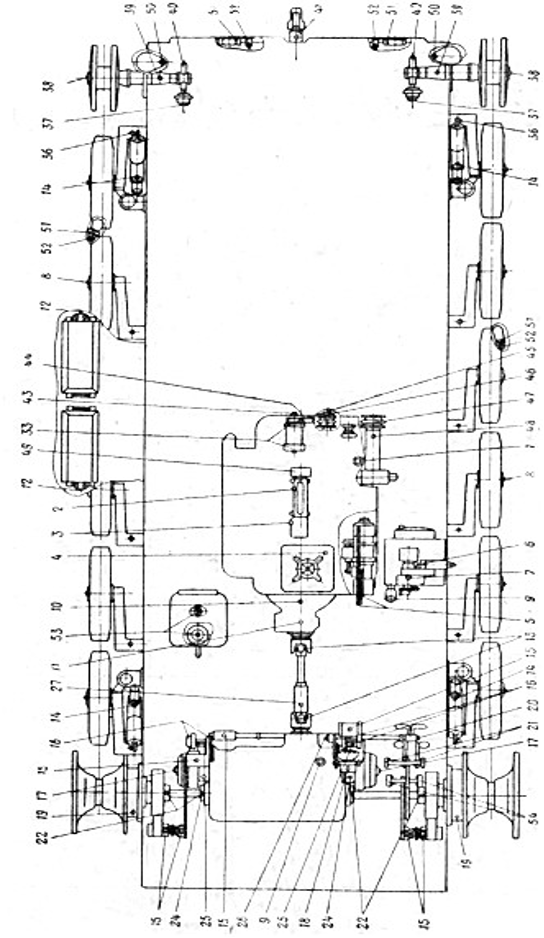
\includegraphics[height=0.95\textheight]{src/appendix_first.png}
    \caption{Схема смазки МТЛБ}
    \label{appendix_first}
\end{figure}


\begin{figure}
    \centering
    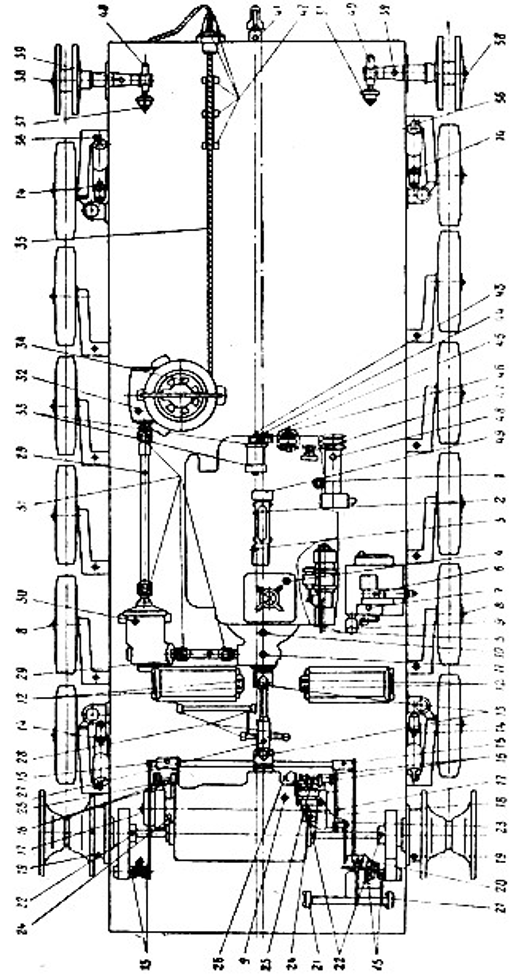
\includegraphics[height=0.95\textheight]{src/appendix_second.png}
    \caption{Схема смазки МТЛБ}
    \label{appendix_second}
\end{figure}

% Размеры колонок
\newcommand{\PointNumberSize}{1.1cm}
\newcommand{\PointNameSize}{1.8cm}
\newcommand{\PointCountSize}{1.53cm}
\newcommand{\TOSize}{1.5cm}
\newcommand{\AdditionalSize}{5cm}

\newcommand{\doublecolumn}[1]{\multicolumn{2}{m{\dimexpr \TOSize * 2 + 2\tabcolsep \relax}|}{#1}}
\newcommand{\triplecolumn}[1]{\multicolumn{3}{m{\dimexpr \TOSize * 3 + 4\tabcolsep \relax}|}{#1}}
\newcommand{\fullcolumn}[1]{\multicolumn{7}{>{\tc}m{\dimexpr \PointNumberSize + \PointNameSize + \PointCountSize + \TOSize * 3 + \AdditionalSize + 12\tabcolsep}}{\textbf{#1}}}

\newcommand{\doubleNameRaw}[1]{\multirow{2}{\PointNameSize}{\tc #1}}

\begin{scriptsize}
\begin{landscape}
\begin{longtable}{
    >{\tc}m{\PointNumberSize}|
    >{\tc}m{\PointNameSize}|
    >{\tc}m{\PointCountSize}|
    >{\tc}m{\TOSize}|
    >{\tc}m{\TOSize}|
    >{\tc}m{\TOSize}|
    m{\AdditionalSize}}

    \multirow{2}{\PointNumberSize}{\tc № точки смазки}  & \multirow{2}{\PointNameSize}{\tc Наименование точек смазок} &\multirow{2}{\PointCountSize}{\tc Количество точек смазок}   & \triplecolumn{\tc Техническое обслуживание} & \multirow{2}{\AdditionalSize}{\tc Дополнительные указания} \\
    \cline{4-6}
                    &   &  & ежедневное    &   №1    &   №2    & \\
    \hline\endhead
    \fullcolumn{\tc Масло Дс-11 (ГОСТ~8581-63), Дп-11 (ГОСТ~5304-54)~--- летом (при~температуре воздуха выше + 5°С),} \\
    \fullcolumn{\tc Дс-8 (ГОСТ~8581-63), Дп-8 (ГОСТ~5304-54)~--- зимой (при~температуре воздуха ниже + 5°C)} \\
    \hline
    \multirow{2}{*}{1} & \doubleNameRaw{Система смазки двигателя} & \multirow{2}{*}{1} & \triplecolumn{Проверить уровень масла в~картере двигателя, при~необходимости дозаправить} & При~дозаправке снять крышку с~заливной горловины, вставить воронку с~сеткой и~долить масло до~метки В на~щупе. \\
    & & & && Заменить масло & При~замене сразу~же после остановки двигателя слить масло из~картера двигателя и~масляного фильтра предварительной очистки. Промыть масляный фильтр налить масло в~поддон до~метки В на~щупе. \\
    \hline

    \multirow{2}{*}{2} & \doubleNameRaw{Топливный насос} & \multirow{2}{*}{1} & \triplecolumn{Проверить уровень масла в~корпусе топливного насоса, при~необходимости дозаправить} & При~дозаправке вывернуть пробку заливного отверстия и~долить масло до~верхней метки на~щупе.\\
    & & & && Через одно ТО-2 заменить масло & Заменить масло при~каждом снятии насоса с~двигателя \\
    \hline

    \multirow{2}{*}{3} & \doubleNameRaw{Картер регулятора топливного насоса} & \multirow{2}{*}{1} & \triplecolumn{Проверить уровень масла, при~необходимости дозаправить} & При~дозаправке вывернуть пробку заливного отверстия и~долить масло до~верхней метки на~щупе \\
    & & & && Через одно ТО-2 заменить масло & При~замене слить старое масло и~залить свежее до~требуемого уровня \\
    \hline
    
    5 & Подшип\-ники стартера & 3 & --- & --- & Через 500~ч работы двигателя или~при~ремонте смазать & Залить \range{10}{15} капель масла в~масленки стартера, в~средний и~задний подшипники залить по~30 капель масла \\ 
    \hline    \fullcolumn{Масло МТ-16л (ГОСТ~6360-58), летом и~зимой} \\
    \hline
    
    4 & Воздухо\-очиститель & 1 & \triplecolumn{Через \range{25}{30}~ч работы двигателя в~особо пыльных дорожных условиях. Через 50~ч в~условиях нормальной запыленности} & Фильтрующие кассеты тщательно промыть в~чистом дизельном топливе и~просушить. Две верхние кассеты пропитать маслом МТ-16п и~дать ему стечь до~прекращения каплепадения\\
    \hline
    
    \multirow{2}{*}{8} &  \doubleNameRaw{Подшип\-ники опорных катков} &  \multirow{2}{*}{12} & --- & \doublecolumn{Проверить уровень масла, при~необходимости дозаправить} & При~дозаправке вывернуть пробку контрольного отверстия и~долить масло \\
    & & & && Через одно ТО-2 заменить масло & При~замене вывернуть пробку сливного отверстия и~слить масло, промыть полость подшипников дизельным топливом и~залить свежее масло до~появления его из~контрольного отверстия. После преодоления водных препятствий проверить наличие воды в~масле, при~обнаружении следов воды масло заменить\\
    \hline
    
    \multirow{2}{*}{9} & \doubleNameRaw{ Главная передача и~масляный бак главной передачи} & \multirow{2}{*}{2} & --- & \doublecolumn{Проверить уровень масла, при~необходимости дозаправить} & При~дозаправке снять пробку заливной горловины масляного бака и~долить масло до~верхней зиговки заливной горловины \\
    & & & && Через одно ТО-2 заменить масло & При~замене слить масло из~масляного бака и~главной передачи сразу~же после остановки транспортера-тягача и~залить в~бак свежее масло до~верхней зиговки заливной горловины и~10~л в~главную передачу. Запустить двигатель, поработать \range{1}{2}~мин вхолостую и~при~необходимости дозаправить до~верхней зиговки заливной горловины бака. Масло МТ-4п (ГОСТ~6360-58) применять зимой в~районах эксплуатации с~особо низкими температурами воздуха (ниже $-$\celc{25}), а~также в~районах Крайнего Севера в~течение всего года \\
    \hline
    
    \multirow{2}{*}{11} & \doubleNameRaw{Промежу\-точный редуктор} & \multirow{2}{*}{1} & --- & \doublecolumn{Проверить уровень масла, при~необходимости дозаправить} & При~дозаправке вывернуть пробку и~долить масло до~уровня верхней метки на~щупе\\
    & & & && Через одно ТО-2 заменить масло & При~замене слить масло сразу~же после остановки транспортера-тягача и~залить свежее масло до~уровня верхней метки на~щупе \\
    \hline
    
    13 & Крестовины центрального карданного вала & 2 & --- & \doublecolumn{\tc Смазать} & Очистить масленку от~грязи и~нагнетать смазку до~появления свежей смазки из~предохранительного клапана\\ 
    \hline
    
    \multirow{2}{*}{19} &  \doubleNameRaw{Бортовые передачи} &  \multirow{2}{*}{2} & --- & \doublecolumn{Проверить уровень масла, при~необходимости дозаправить} & При~дозаправке вывернуть пробку контрольного отверстия и~долить масло до~уровня контрольного отверстия\\
    & & & && Через одно ТО-2 заменить масло & При~замене слить масло сразу~же после остановки транспортера-тягача и~залить свежее масло до~уровня контрольного отверстия. При~температуре ниже $-$\celc{30} применять масло МТ-14п (ГОСТ~6360-58). Заменители масла МТ-16п: летом~--- масло трансмиссионное автотракторное летнее; зимой~--- зимнее (ГОСТ~542-50) \\
    \hline
    
    30 & Реверс-редуктор лебедки & 1 & \triplecolumn{Через 100 подтягиваний и~50 спусков} & Вывернуть пробку и~долить масло до~уровня верхней метки на~щупе. Заменитель масла МТ-16п: масло АК-10 (ГОСТ~1862-63) летом и~зимой\\
    \hline
    
    31 & Крестовины карданов привода лебедки & 4 & \triplecolumn{Через 25 полных подтягиваний} & Рычажно-плунжерным шприцем с~насадкой нагнетать масло через крестовины кардана до~появления свежей смазки из~контрольного клапана. Заменители масла МТ-16п: летом~--- масло трансмиссионное автотракторное летнее, зимой~--- зимнее (ГОСТ~542-50)\\
    \hline
    
    32 & Лебедка & 1 &  \triplecolumn{Через 100 подтягиваний и~50 спусков} & Вывернуть пробку и~долить масло до~уровня верхней метки на~щупе. Заменитель масла МТ-16п: масло трансмиссионное автотракторное летнее~--- летом, зимнее~--- зимой (ГОСТ~542-50)\\
    \hline
    
    38 & Подшип\-ники направляющих колес & 2 & --- &  \doublecolumn{Проверить уровень масла, при~необходимости дозаправить} & При~дозаправке вывернуть пробку контрольного отверстия и~долить масло \\
    \hline
    
    \multirow{2}{*}{48} & \doubleNameRaw{Редуктор вентиля\-тора} & \multirow{2}{*}{1} & --- & \doublecolumn{Проверить уровень масла, при~необходимости дозаправить} & При~дозаправке отвернуть пробку со~щупом и~долить масло до~уровня метки на~щупе \\
    & & & && Заменить масло & При~замене отвернуть пробку, слить старое масло и~залить свежее до~уровня метки на~щупе \\
    \hline
    
    \newpage
    \fullcolumn{Смазка 1-13 жировая (ГОСТ~1631-61) или~ЦИАТИМ-201 (ГОСТ~6267-59) летом и~зимой} \\
    \hline

    10 & Муфта выключения главного фрикциона & 1 & \triplecolumn{\tc Смазать} & Очистить масленку и~заправить смазку, сделав \range{два}{три} нагнетания шприцем. При~движении в~тяжелых дорожных условиях при~частом переключении передач смазывать муфту ежедневно\\
    \hline
    
    16 & Подшип\-ники валиков кулаков мостиков управления & 4 & --- & --- & Через одно ТО-2 заменить смазку & Разобрать мостики управления, очистить подшипники от~старой смазки и~заложить новую. Заменитель смазки 1-13: консталин жировой УТ-1 (ГОСТ~1957-52) летом и~зимой\\
    \hline
    
    17 & Подшип\-ники ведущих барабанов фрикционов механизмов поворота & 2 & \triplecolumn{\tc Смазать} & Очистить масленку от~грязи и~сделать \range{пять}{шесть} нагнетаний шприцем. Заменитель смазки 1-13: консталин жировой УТ-1 (ГОСТ~1957-52) летом и~зимой\\
    \hline

    18 & Колонка переключения передач & 2 & \triplecolumn{\tc Смазать} & Очистить масленку от~грязи и~нагнетать до~появления свежей смазки из-под поводков. Заменитель смазки 1-13: консталин жировой УТ-1 (ГОСТ~1957-52) летом и~зимой\\
    \hline
    
    22 & Шлицевые соединения зубчатых карданов главной передачи & 4 & \triplecolumn{\tc Смазать} & Очистить масленку от~грязи и~нагнетать до~появления свежей смазки из-под уплотнений. \\
    \hline
    
    24 & Подшип\-ники механизмов выключения фрикционов и~механизмов поворота & 2 & \triplecolumn{\tc Смазать} & Очистить масленку от~грязи и~нагнетать до~появления свежей смазки из-под колец. При~движении на~плаву заправлять ежедневно. Заменитель смазки 1-13: консталин жировой УТ-1 (ГОСТ~1957-52) летом и~зимой\\
    \hline
    
    25 & Мостики управления & 2 & \triplecolumn{\tc Смазать} & Очистить масленку от~грязи и~сделать \range{пять}{шесть} нагнетаний шприцем. Заменитель смазки 1-13: консталин жировой УТ-1 (ГОСТ~1957-52) летом и~зимой\\
    \hline
    
    43 & Подшип\-ники шкива привода компрессора & 1 & --- & --- & Смазать & Очистить масленку от~грязи и~сделать \range{три}{четыре} нагнетания шприцем\\ 
    \hline
    
    44 & Подшип\-ники натяжного ролика привода генератора & 2 & \triplecolumn{\tc Смазать} & Очистить масленку от~грязи сделать \range{три}{четыре} нагнетания шприцем. Заменитель смазки 1-13: консталин жировой УТ-1 (ГОСТ~1957-52) летом и~зимой\\
    \hline

    45 & Подшип\-ники натяжного ролика привода компрессора & 1 & --- & --- & Смазать & Очистить масленку от~грязи и~сделать \range{четыре}{пять} нагнетаний шприцем\\ 
    \hline
    
    46 & Подшип\-ники натяжного ролика ремня вентилятора & 1 & \triplecolumn{\tc Смазать} & Очистить масленку от~грязи и~сделать \range{пять}{шесть} нагнетаний шприцем. Заменитель смазки 1-13: консталин жировой УТ-1 (ГОСТ~1957-52) летом и~зимой\\
    \hline
    
    47 & Подшип\-ники водяного насоса & 1 & --- & \doublecolumn{\tc Смазать} & Очистить масленку от~грязи и~нагнетать до~появления свежей смазки из~верхнего контрольного отверстия\\ 
    \hline    \fullcolumn{Солидол синтетический (ГОСТ~4366-64) летом и~зимой} \\
    \hline

    12 & Клеммы аккумуляторных батарей & 4 & --- & \doublecolumn{\tc Смазать} & Клеммы очистить от~окиси, закрепить на~них провода и~смазать клеммовые соединения \\
    \hline
    
    20 & Валик рычагов управления & 1 & --- & \doublecolumn{\tc Смазать} & Очистить масленку от~грязи и~нагнетать до~появления свежей смазки в~торцах кронштейна\\
    \hline
    
    23 & Переходный валик тяги левого мостика управления & 1 & --- & --- & Смазать & То~же\\
    \hline
    
    26 & Валик тяги главного фрикциона & 1 & --- & --- & Смазать & То~же\\
    \hline
    
    36 & Кронштей\-ны подвески & 12 & --- & --- & Смазать & Вывернуть пробку, ввернуть шланг и~сделать \range{два}{три} нагнетания шприцем\\
    \hline

    37 & Подшип\-ники натяжных винтов направляющих колес & 2 & --- & \doublecolumn{\tc Смазать} & Очистить масленку от~грязи и~сделать \range{три}{четыре} нагнетания шприцем \\
    \hline

    40 & Натяжные винты направляющих колес & 2 & --- & \doublecolumn{\tc Смазать} & Очистить винт от~грязи и~смазать \\
    \hline

    41 & Тягово-сцепной прибор & 1 & --- & \doublecolumn{\tc Смазать} & Очистить масленку от~грязи и~сделать \range{пять}{шесть} нагнетаний шприцем\\
    \hline

    15 & Подшип\-ники передаточного вала и~кронштейнов остановочных тормозов & 6 на~МТЛ, 7~на~МТ-ЛБ & --- & --- & Смазать & Очистить масленку от~грязи и~сделать \range{три}{четыре} нагнетания шприцем\\
    \hline

    52 & Механизмы запирания бортовых лючков & 4 & --- & --- & Заменить смазку & Разобрать механизм запирания бортовых лючков, удалить старую смазку и~заложить новую \\
    \hline

    51 & Шаровые опоры бортовых лючков & 4 & --- & --- & Заменить смазку & Разобрать шаровую опору бортовых лючков, удалить старую смазку и~заложить новую \\
    \hline
    
    50 & Механизмы запирания крышек заливных горловин топливных баков & 2 & --- & --- & Заменить смазку & Разобрать механизм запирания крышек заливных горловин, удалить старую смазку и~заложить новую\\
    \hline

    39 & Кронштейн направляющих колес & 2 & --- & --- & Через одно ТО-2 смазать & Очистить масленку от~грязи и~сделать \range{15}{20} нагнетаний шприцем\\
    \hline

    27 & Шлицевое соединение центрального карданного вала & 1 & --- & --- & Через одно ТО-2 смазать & Разобрать шлицевое соединение карданного вала, удалить старую смазку и~заложить новую\\
    \hline

    21 & Подшипники валика педали главного фрикциона & 2 & --- & --- & Через одно ТО-2 заменить смазку & Разобрать валик педали главного фрикциона, очистить подшипники от~старой смазки и~заложить новую\\
    \hline

    54 & Подшипники промежуточного вала левого рычага управления & 2 & --- & --- & Через одно ТО-2 заменить смазку & Разобрать промежуточный вал, очистить подшипники от~старой смазки и~заложить новую\\
    \hline
    
    53 & Сиденье поворотное & 2 & --- & --- & Через одно ТО-2 заменить смазку & Снять сиденье, очистить полости кронштейнов от~старой смазки и~заполнить новой смазкой \\
    \hline
    
    29 & Шлицевые соединения карданных валов привода лебедки & 2 & \triplecolumn{Через 100 полных подтягиваний и~50 спусков смазать} & Очистить масленки от~грязи и~сделать \range{пять}{шесть} нагнетаний шприцем\\
    \hline
    
    42 & Датчик ограничителя усилия на~тросе лебедки и~выводное устройство троса лебедки & 5 & \triplecolumn{Через \range{20}{25} полных подтягиваний смазать} & Очистить масленки от~грязи и~сделать \range{три}{четыре} нагнетания шприцем\\
    \hline
    
    34 & Подшипники ступицы барабана лебедки & 1 & \triplecolumn{Через \range{20}{25} полных подтягиваний смазать} & Очистить масленки от~грязи и~сделать \range{три}{четыре} нагнетания шприцем\\
    \hline
    
    28 & Подшипники валиков привода управления лебедкой & 4 & \triplecolumn{Через 100 полных подтягиваний и~50 спусков смазать} & Разобрать привод, удалить старую смазку и~заполнить новой \\
    \hline
    
    35 & Трос лебедки & 1 & \triplecolumn{Каждый раз при~пользовании лебедкой смазать} &  После окончания работы очистить трос от~грязи и~при~наматывании на~барабан смазать\\
    \hline

    \fullcolumn{Смазка ЦИАТИМ-203 (ГОСТ~8773-63)}\\
    \hline

    49 & Муфта опережения впрыска топлива & 1 & \triplecolumn{При~ремонте муфты заменить смазку} & После разборки муфты удалить старую смазку и~заложить новую\\
    \hline

    \fullcolumn{Смазка Л3-158 (ВТУ ТН3 №100-61), ЦИАТИМ-221 (ГОСТ~9433-60) или~ЦИАТИМ-201 (ГОСТ~6267-59)} \\
    \hline

    33 & Подшипники генератора & 2 & --- & --- & Через 1000~ч работы двигателя заменить смазку & Снять генератор с~двигателя, разобрать его, удалить старую смазку и~промыть шарикоподшипники в~бензине. Заложить в~подшипники свежую смазку. Собрать генератор и~установить на~двигатель\\
    \hline    \fullcolumn{Смесь из~50\% трансформаторного масла (ГОСТ~982-68) и~50\% турбинного масла (ГОСТ~32-53)}\\
    \hline

    14 & Гидроамор\-тизаторы & 4 & --- & --- & Дозаправить & Дозаправить гидроамортизатор без~его снятия. Очистить гидроамортизатор от~грязи, отвернуть пробку компенсационной камеры и~линейкой проверить уровень жидкости. Расстояние от~дна компенсационной камеры до~уровня жидкости должно быть: 
    \begin{itemize}
        \item при~загруженном транспорте~--- \range{140}{150}~\textit{мм};
        \item при~разгруженном транспорте: 
            \begin{itemize}
            \item передние \range{148}{154} \textit{мм};
            \item задние  \range{128}{132} \textit{мм}.
            \end{itemize}
    \end{itemize}\\
    \hline
    
    \fullcolumn{Смесь из~70\% масла дизельного Дс-8 (ГОСТ~8581-63) с~присадкой и~30\% дизельного топлива (ГОСТ~4749-49) марки ДЗ, летом и~зимой}\\
    \hline 

    6 & Редуктор подогревателя & 1 & \triplecolumn{Через \range{10}{15}~ч работы редуктора или~через \range{20}{30} пусков дозаправить (при~очередном ТО-1)} & Отвернуть пробку заливного и~контрольного отверстия залить смесь до~уровня контрольного отверстия\\
    \hline 

    7 & Опора верхнего валика редуктора подогревателя & 1 & \triplecolumn{Через \range{10}{15}~ч работы редуктора или~через \range{20}{30} пусков дозаправить (при~очередном ТО-1)} & Отвернуть пробку и~залить \range{2}{3}~см$^3$ смеси\\
    \hline

\end{longtable}
\end{landscape}
\end{scriptsize}


\newcommand{\itemshort}[2]{
\noindent
#1 \dotfill \makebox[1cm][r]{#2} 
}

\newcommand{\itemlong}[2]{
\noindent
#1 \dotfill \makebox[2.3cm][r]{#2} 
}


\chapter{Емкостные данные}

\itemshort{Топливная система}{550} 

\itemshort{Правая группа баков}{272} 

\itemshort{Левая группа баков}{278}

\itemshort{Система смазки двигателя}{32}

\itemshort{Система охлаждения}{55}

\itemshort{Бачок топливной системы подогрева}{5}

\itemshort{Бидон запасной с~маслом (канистра)}{10}

\itemshort{Главная передача}{10}

\itemshort{Масляный бак главной передачи}{11}

\itemshort{Лебедка (картер)}{7,6}

\itemlong{Бортовая передача (две)}{1,7 каждая}

\itemlong{Ступицы направляющих колес (две)}{0,5 каждая}

\itemlong{Ступицы опорных катков (двенадцать)}{0,55 каждая}

\itemlong{Гидроамортизатор (четыре)}{0,9 каждый}

\itemshort{Промежуточный редуктор}{0,6}

\itemshort{Реверс-редуктор лебедки}{1,1}

\itemshort{Редуктор подогревателя}{0,10}

\itemshort{Редуктор вентилятора}{0,20}

\itemshort{Топливный насос}{0,20}

\itemshort{Картер регулятора топливного насоса}{0,15}


\end{document}